\documentclass{article}      	% Style of the document                     
\usepackage{fullpage}
\usepackage{amsmath}     	   	% Maths                                          
\usepackage[utf8]{inputenc}	% UTF-8 characters                                               
\usepackage[T1]{fontenc}    	% Tuki ääkkösille (Finnish names don't cause problems)                                            
\usepackage{parskip}        		% Linebreak between paragraphs                
\usepackage{svg}
\usepackage{graphicx}       		% Graphics package for adding figures                        
\usepackage{epstopdf}       		% Possibility to add *.eps figures
 \usepackage{ dsfont }            % Symbol for real numbers
\usepackage{hyperref}
\usepackage{extarrows}
\usepackage{float}
\usepackage{makeidx}
\usepackage{enumitem}        % possibility to label list items by alphabet
\usepackage[a4paper, top=0.5in]{geometry}
\newcommand{\M}[1]{\ensuremath{\text{\texttt{#1}}}}
\usepackage[
    lambda,
    operators,
    advantage,
    sets,
    adversary,
    landau,
    probability,
    notions,
    logic,
    ff,
    mm,
    primitives,
    events,
    complexity,
    asymptotics,
    keys]{cryptocode}

\usepackage{todonotes}

 \usepackage{amsmath,amsfonts,graphicx,amssymb,amsthm}
\mathchardef\mhyphen="2D

 %% general
\mathchardef\mhyphen="2D
\newcommand{\fdv}{\mathcal{F}}
\newcommand{\tdv}{\mathcal{T}}
\newcommand{\vdv}{\mathcal{V}}
\newcommand{\cX}{\mathcal{X}}
\newcommand{\cF}{\mathcal{F}}
\newcommand{\cG}{\mathcal{G}}
\newcommand{\ID}{\mathcal{I}}
\newcommand{\bits}[1][]{\{0,1\}^{#1}}
\renewcommand{\vec}[1]{\mathbf{#1}}
\newcommand{\mat}[1]{\mathbf{#1}}
\newcommand{\inner}[2]{\langle #1, #2 \rangle}
\newcommand{\transpose}{\mathtt{T}}
\newcommand{\round}[1]{\lfloor #1 \rceil}
\renewcommand{\dist}{\mathsf{dist}}
\renewcommand{\Pr}[2][]{{\text{Pr}_{#1}\left[#2\right]}}
\newcommand{\Exp}[2][]{{\mathbb{E}_{#1}\left[#2\right]}}
\newcommand{\mathcm}[2][1cm]{\hspace{#1}{\mbox{/\!\!/ } \text{\scriptsize#2}}}

%% lattice problems
\newcommand{\SIS}{\mathsf{SIS}}
\newcommand{\ISIS}{\mathsf{ISIS}}
\newcommand{\nfSIS}{\mathsf{nfSIS}}
\newcommand{\dSIS}{\mathsf{dSIS}}
\newcommand{\LWE}{\mathsf{LWE}}
\newcommand{\nfLWE}{\mathsf{nfLWE}}
\newcommand{\nfdLWE}{\mathsf{nfdLWE}}
\newcommand{\sLWE}{\mathsf{sLWE}}
\newcommand{\dLWE}{\mathsf{dLWE}}
\newcommand{\SVP}{\mathsf{SVP}}
\newcommand{\CVP}{\mathsf{CVP}}
\newcommand{\SIVP}{\mathsf{SIVP}}
\newcommand{\GapSVP}{\mathsf{GapSVP}}
\newcommand{\BDD}{\mathsf{BDD}}
\newcommand{\NTRU}{\mathsf{NTRU}}
\newcommand{\sNTRU}{\mathsf{sNTRU}}
\newcommand{\dNTRU}{\mathsf{dNTRU}}

%% lattice macros
\newcommand{\TT}{\mathbb{T}}
\newcommand{\ring}{\mathcal{R}}
\newcommand{\lattice}{\mathcal{L}}
\newcommand{\piped}{\mathcal{P}}
\newcommand{\ball}{\mathcal{B}}
\newcommand{\Hyb}{\mathsf{Hyb}}
\newcommand{\lspan}{\mathsf{span}}
\newcommand{\rank}{\mathsf{rank}}
\newcommand{\lsb}{\mathsf{LSB}}
\newcommand{\pubparam}{\mathsf{pp}}

%% group macros

%% syntax
\newcommand{\mpk}{\mathsf{mpk}}
\newcommand{\msk}{\mathsf{msk}}
\newcommand{\msg}{\mathsf{msg}}
\newcommand{\rnd}{\mathsf{rnd}}
\newcommand{\ctxt}{\mathsf{ctxt}}
\newcommand{\com}{\mathsf{com}}
\newcommand{\td}{\mathsf{td}}
\newcommand{\id}{\mathsf{id}}
\newcommand{\stmt}{\mathsf{stmt}}
\newcommand{\wit}{\mathsf{wit}}
\newcommand{\tx}{\mathsf{tx}}
\newcommand{\aux}{\mathsf{aux}}
\newcommand{\ek}{\mathsf{ek}}

\newcommand{\Setup}{\mathsf{Setup}}
\newcommand{\Commit}{\mathsf{Com}}
\newcommand{\TrapGen}{\mathsf{TrapGen}}
\newcommand{\SampD}{\mathsf{SampD}}
\newcommand{\SampPre}{\mathsf{SampPre}}
\newcommand{\Prove}{\mathsf{Prove}}
\newcommand{\Verify}{\mathsf{Verify}}
\newcommand{\val}{\mathsf{val}}

%% primitive/scheme name
\newcommand{\PKE}{\mathsf{PKE}}
\newcommand{\LTDF}{\mathsf{LTDF}}
\newcommand{\rsagen}{\mathsf{RSAGen}}
\newcommand{\rsa}{\mathsf{RSA}}
\newcommand{\LHE}{\mathsf{LHE}}
\newcommand{\CS}{\mathcal{CS}}
\newcommand{\NTRUEncrypt}{\mathsf{NTRUEncrypt}}

%% others
\newcommand{\oracle}{\mathcal{O}}
\newcommand{\pcas}{~\mathbf{as}~}

\newcommand{\polylog}[1][\secpar]{\mathsf{polylog}(#1)}

\newcommand{\indrsidcpa}{\mathrm{IND\$}\mhyphen\mathrm{sID}\mhyphen\mathrm{CPA}}
%\newcommand{\oplus}{\, \texttt{XOR} \,} % shorthand for typing the XOR operator in mathmode
\usepackage{tikz}
\usetikzlibrary{decorations.pathreplacing}
\usetikzlibrary{decorations.pathmorphing}


\definecolor{cgreen}{RGB}{0, 153, 51}
\definecolor{cblue}{RGB}{0, 102, 204}
\definecolor{cyellow}{RGB}{255, 204, 0} 
\definecolor{cred}{RGB}{204, 51, 0} 

\newcommand{\commentline}[2]{%
    \tikz[remember picture, overlay]{
        \node [black,anchor=west,xshift=10pt] at (#1) {#2};
    }
}

\newcommand{\blockcomment}[3]{%
    \tikz[remember picture, overlay]{
        \draw [decorate,decoration={lineto,amplitude=10pt,mirror,raise=4pt},yshift=0pt,very thick,{#3}] 
        (#1) -- (#2) node [black,midway,xshift=10pt] {};
    }
}



\usepackage{biblatex}
\addbibresource{references.bib}

\begin{document}         
\author{Lorenzo Tucci}
\title{Atomic swaps from timed commitments}

\maketitle

\tableofcontents
\newpage
\section{Introduction}

Blockchains are distributed ledgers managed by peer-to-peer computer networks called $nodes$, which collectively adhere to a consensus protocol to add and validate record of transactions in a decentralized, permissionless and trustless manner. \\
Given the increasing number of blockchain systems, one of the most critical features in the cryptocurrency landscape is blockchain interopability, particularly the ability to exchange heterogeneous assets between different ledgers while maintining the trustless and decentralized properties of the individual chains. 

An atomic cross-chain swap is an exchange of assets across different blockchains between two users without any additional trust assumption. 
Consider two ledgers $\mathbb{A}$ and $\mathbb{B}$, where Alice holds assets $a$ in $\mathbb{A}$ and Bob holds assets $b$ in $\mathbb{B}$. We want to ensure that Alice transfers her assets $a$ in $\mathbb{B}$ to Bob if and only if Bob transfers his asset $b$ to Alice in $\mathbb{B}$.

The word \textit{atomic} implies that the protocol execution can result in only two possible outcomes: \\
1) the asset swap is successful, resulting in Bob owning $a$ in $\mathbb{A}$ and Alice owning $b$ in $\mathbb{B}$ \\
2) the swap aborts, leading to a refund of the assets and thus in Alice retaining $a$ in $\mathbb{A}$ and Bob $b$ in $\mathbb{B}$ 

In order to realize such functionality, protocols follow a standard blueprint where funds from a party are placed in a frozen state from which the assets either will be swapped to the counter-party or refunded after a certain timeout. \\
Protocols can either rely on the scripting language of the underlying blockchain using timelocks or on cryptographic timed commitments, where secrets are commited under a cryptographic puzzle that can be solved after a certain number of sequential operations. 
While timelocks can be an effective building block in order to a realize an atomic swap protocol, the set of blockchains supporting such functionality is restricted, and it excludes privacy chains such as Monero or Zcash. Furthermore, transactions incure in higher execution costs due to scripting, and generate additional on-chain data that can potentially compromise privacy. \\
On the other hand, cryptographic puzzles impose a computation burden on users, which are incentivized to make worst-case estimates for the counterparty's computational power that can be orders of magnitude faster when accounting for novel algorithms \cite{squaring_algo} and application-specific integrated circuits (ASIC) \cite{squaring_asic}. \\
This results in a potentially impractical protocol, as parties may need to uninterruptedly compute a force opening for a significant amount of time on conventional hardware.

In this work we investigate whether such a computational burden can be restricted to one party, acting as an exchange server, by using a single refund timeout. Furthermore, we evaluate whether existing protocols take into account different blockchain confirmation time when setting timeouts for cryptographic timed commitments to prevent potential transaction racing attacks.

%\todo[inline]{TODO starts}
%\begin{itemize}
%    \item General description of problem (swapping), motivations, etc.
%    \item Introduce Universal Atomic Swaps (UAS) and its building blocks, briefly discuss how the protocol works, and highlight the issue of both parties needing to solve a VTS
%    \item The ``our contribution'' subsection: e.g. ``We propose an alternative construction ... we provide an open source implementation ...''
%    \item (Not so) Related work (subsection or section): Other ways to get atomic swaps, e.g. TEE, relays, HTLC, ...
%    \item \url{https://ieeexplore.ieee.org/stamp/stamp.jsp?tp=&arnumber=9797357&tag=1} provides an alternative construction of atomic swap without a trusted setup but requiring special chain verification logic. To capture this, we want to abstract away the time-lock functionality so that it can be implemented in different ways, e.g. with TLP, custom chain logic, or new ways like commit transactions.
%    \item Add comments to pseudocode. Split chunks of the protocol to be run in parallel into subroutines. Give more descriptive variable names (e.g. instead of $P_0, P_1, T_0, T_1$)
%\end{itemize}
%
%\todo[inline]{TODO ends}

\subsection{Existing solutions}

%\begin{table}[H]
%\centering
%\begin{tabular}{|c|c|c|c|}
%\hline
%\textbf{Type} & \textbf{Trustless} & \textbf{Transparent} & \textbf{Scriptless} \\
%\hline
%TEE [BJZLZBDJ'17] & & \checkmark & \checkmark \\
%\hline
%HTLC [Gugger '20] & \checkmark & &\\
%\hline
%Relays [LMP'21] & \checkmark & &  \\
%\hline
%Universal [MTS'20] & \checkmark & \checkmark & \checkmark \\
%\hline
%\end{tabular}
%\caption{Properties comparison of different atomic swaps protocol}
%\end{table}
%\subsubsection{Hashed Timelock Contract (HTLC)}

\subsubsection{Hash Time Lock Contracts}

By utilizing a blockchain's scripting language and timelock functionalities it is possible to create a script that acts as a timed escrow, which can be claimed if certain condition are met or refunded upon expiration.
Specifically, a Hash Time Lock Contract (HTLC) is defined by a tuple $(\mathsf{amnt_a}, h, T, \mathsf{pk_0}, \mathsf{pk_1})$ where 
\begin{itemize}
	\item $\mathsf{amnt_a}$ denotes the amount of $\mathsf{a}$ assets to be exchanged
	\item $h$ is a hash value
	\item $T$ the timeout
	\item $\mathsf{pk_{tx}}$ and $\mathsf{pk_{rx}}$ the public key addresses of two users
\end{itemize}

The HTLC transfers $\mathsf{amnt_a}$ to $\mathsf{pk_1}$ if invoked before timeout $T$ with input value $r$ such that $\mathcal{H}(r) = h$. 
If the contract is invoked after timeout $T$, it refunds the assets $\mathsf{amnt_a}$ to $\mathsf{pk_0}$ unconditionally.

Using HTLCs as a building block, an atomic swap protocol can be constructed as follows: \\
1) Alice chooses $r$, computes $h = \mathcal{H}(r)$, transfers $\mathsf{amnt_a}$ into an $(\mathsf{amnt_a}, h, T_0, \mathsf{pk_0}, \mathsf{pk_1})$ on blockchain $\mathbb{A}$ and sends $h,T$ to Bob. \\
2) Bob finishes the setup of the exchange by choosing a time $T_1 < T_0$ and transferring his $\mathsf{amnt_b}$ assets into an HTLC$(\mathsf{amnt_b}, h, T_1, \mathsf{pk_{tx}}, \mathsf{pk_{rx}})$ on blockchain $\mathbb{B}$. 

Bob cannot claim the HTLC yet as $r$ is only known by Alice, thus there are only two possible outcomes:
\begin{itemize}
\item Alice claims the HTLC on $\mathbb{B}$ before $T_0$, effectively revealing $r$ to Bob (and anyone observing $\mathbb{B}$), Bob can then proceed to compute $h = \mathcal{H}(r)$ to claim the counterpart HTLC on chain $\mathbb{A}$ 
\item Alice does not claim the HTLC on $\mathbb{B}$ in time and thus Bob cannot claim the HTLC on $\mathbb{A}$. After the respective timeouts they can refund the assets by invoking the contracts.
\end{itemize}

This functionality can be achieved without requiring complex scripting functionality \cite{h4sh3d} using semi-scriptless scripts. \\
Additionally, a similar protocol can also be realized even if only one blockchain supports HTLCs or timelocks, as realized in the protocol proposed by Gugger \cite{h4sh3d} in the Monero counterpart.

%\todo[inline]{explain (splitting secret key, BTC party needs to move first)}

%\subsubsection{Relays}
%Another strategy to achieve atomic swaps relies on relays. Relays are abstractions (in general a smart contract or a script) hosted on some
%chain $\mathbb{B}_a$ that has light client like verification capabilities over chain $\mathbb{B}_b$. For each new block appended to chain $\mathbb{B}_a$,
%the block header is passed on to the relay on chain $\mathbb{B}_b$. \\
%The relay itself implements the standard verification procedure of chain $\mathbb{B}_a$’s consensus algorithm and can therefore verify the
%validity of the block. Once the proof of work has been verified,
%in the case of a Proof of Work (or PoW) blockchain, or the
%two-thirds of validators signatures, in the case of a Byzantine
%Fault Tolerant (or BFT) blockchain, it is possible to verify any
%transaction of chain $\mathbb{B}_a$ from chain $\mathbb{B}_b$. With light client
%like verification capabilities of chain $\mathbb{B}_a$ from chain $\mathbb{B}_b$,
%we can imagine the following scenario. Bob has X assets of
%chain $\mathbb{B}_b$. He is willing to exchange them for Y assets of
%chain $\mathbb{B}_a$.  \\
%    Bob sets up a smart contract SC1 and locks his
%assets in it (1). This smart contract SC1 is set to release the
%assets to anyone providing the proof that they made a payment
%of Y assets of chain $\mathbb{B}_a$ to Bob’s address. Alice, who is
%interested in this trade, transfers Y assets to Bob’s address (2).
%She retrieves the transaction hash tx and provide it to SC1 (3).
%SC1 calls the relay and asks for verification of transaction tx
%(4). The relay verifies that the transfer has taken place and if
%so, returns ok to SC1 (5). On receiving the answer from the
%relay, SC1 transfers the X assets of $\mathbb{B}_b$ to Alice’s address.

%\begin{figure}[H]
%\begin{pchstack}[center, boxed]
%\pseudocode{
%    \textbf{$P_0(pk(0)\:, sk(0)$)} \< \< \textbf{$P_1(pk(1)\:, sk(1))$} \\[0.1\baselineskip ][\hline] 
%    \<\< \\[-0.5\baselineskip ]
%    \< \sendmessage*{<->}{top={{\Gamma_{\mathsf{KeyGen}}(\mathbb{G},G,q)}}, bottom={\xlonggets{} (sk_0(01), pk(01)) \\ (sk_1(01), pk(01)) \xlongrightarrow{} }} \< \\
%    \<\< (C, \pi) \gets \Pi_{\mathsf{VTD}}.\mathsf{Commit}(sk_1, T) \\
%    \< \sendmessageleft*{(C, \pi)} \< \\
%    \mathsf{starts}\: \mathsf{Timeout}(T - \Delta)
%    \<\< \mathsf{starts}\: \mathsf{Timeout}(T - \Delta) \\
%    \mathsf{if}\: \Pi_{\mathsf{VTD}}.\mathsf{Verify}(pk, C, \pi) \neq 1 \\
%    \qquad \mathsf{abort}\\
%    tx_\mathsf{frz} \gets \mathsf{InitTx}(pk(0), pk(01), \mathsf{swp(a)}, \mathbb{A}) \\
%    \sigma_{\mathsf{frz}} \gets \Pi_{\mathsf{DS}}.\mathsf{Sign}(sk(0), tx_\mathsf{frz}) \\
%    \mathsf{PubTx}(\sigma_{\mathsf{frz}}, tx_\mathsf{frz}, \mathbb{A}) \\
%    \mathsf{starts}\: \Pi_{\mathsf{VTD}}.\mathsf{ForceOp}(C) \\
%    \<\< \mathsf{do}\: \mathsf{bal} \gets \mathsf{GetBal}(pk(01), \mathbb{A}) \\
%    \<\< \mathsf{while}\: \mathsf{bal} \neq \mathsf{swp(a)}\\
%    \< \sendmessageleft*{pk(1)} \< \\
%    (pk(10), sk(10)) \gets \Pi_{\mathsf{DS}}.\mathsf{KeyGen}(1^\lambda) \\
%    tx_\mathsf{swp} \gets \mathsf{InitTx}(pk(1), pk(10), \mathsf{swp(b)}, \mathbb{A}) \\
%    \< \sendmessage*{<->}{top={{\Gamma_{\mathsf{Swap}} \qquad \qquad \\ P_0 \xlongrightarrow{} (sk_0(01), tx_\mathsf{swp}) \\ (sk_1(01), sk(1)) \xlonggets{} P_1 }}, bottom={lk := \sigma_{swp}(10) \oplus sk_0(01) \xlongrightarrow{} \\  \xlongleftarrow{} \sigma_{swp}(10) \qquad \qquad  }} \< \\
%    \mathsf{PubTx}(\sigma_{\mathsf{swp(10)}}, tx_\mathsf{frz}, \mathbb{A}) \\
%    \<\< \mathsf{do}\: \sigma_{swp}(10) \gets \mathsf{GetSig}(pk(1), \mathbb{B}) \\
%    \<\< \qquad sk(01) \gets (lk \oplus \sigma_{swp}(10)) + sk_1 \\
%    \<\< \qquad \sigma_{m} \gets \Pi_{\mathsf{DS}}.\mathsf{Sign}(sk(01), 1) \\
%    \<\< \mathsf{while}\: \Pi_{\mathsf{DS}}.\mathsf{Verify}(m, pk, \sigma_{m}) \neq 1 \\
%}
%\end{pchstack}
%\caption{Universal atomic swap protocol execution for a successful swap}
%\end{figure}
%

\subsubsection{Universal Atomic Swaps}


Thyagarajan et al. \cite{uas} introduced one of the first atomic swap protocols substituting blockchain timelocks with a cryptographic primitive. 
The core building block utilized are Verifiable Timed Signatures (VTS) \cite{vts}, which lets a user generate a timed commitment $C$ of a signature $\sigma$ on a message $m$ under a public key $\mathsf{pk}$. The commitment $C $ must hide the signature $\sigma$ for time $\mathsf{T}$ and producing a proof $\pi$ that $C$ contains a valid signature $\sigma$. This ensures that $\sigma$ can be publicly recovered in time $\mathsf{T}$ by anyone who solves the computational puzzle. We note that a similar construction called Verifiable Timed Discretelog (VTD) allows to commit on a dlog value instead of a signature, and can be alternatively used in the protocol.

Let $P_0$ and $P_1$ be two parties where $P_0$ wants to exchange $\mathsf{amnt_a}$ on blockchain $\mathbb{A}$ from their address $\mathsf{pk_{init(\mathbb{A})}}$ for $\mathsf{amnt_b}$ on blockchain $\mathbb{B}$ to $\mathsf{pk_{swp(\mathbb{B})}}$ and vice-versa for $P_1$.

In the setup phase of the protocol, the parties run a 2PC protocol to setup two freeze addresses on the respective chains $\mathsf{pk_{frz(\mathbb{A})}}$ and $\mathsf{pk_{frz(\mathbb{B})}}$, where each party posseses one share of the respective secret keys, e.g. $\mathsf{sk_{frz(\mathbb{A})}} := \mathsf{sk_{frz0}} \oplus  \mathsf{sk_{frz1}}$. \\
Now the parties create a refund transaction transferring back the assets in case of timeout, for $P_0$ we have $\mathsf{tx_{rfnd(\mathbb{A})}}$ refunding $\mathsf{amnt_a}$ from $\mathsf{pk_{frz(\mathbb{A})}}$ to $\mathsf{pk_{init(\mathbb{A})}}$ and similarly for $P_1$ $\mathsf{tx_{rfnd(\mathbb{B})}}$. \\
Each party generates a timed commitment on the signature of the counterparty's refund transaction, where $P_0$ receives a $\mathsf{VTS}$ with commitment $C_0$ and timeout $T_0 = T_1 + \Delta$ and $P_1$ receives a $\mathsf{VTS}$ with commitment $C_1$ and timeout $T_1$. Once both $\mathsf{VTS}$ commitment are verified the parties proceed to transfer the assets to the freeze addresses, assured to retrieve the refund transaction signatures after force opening the commitments with timeouts $T_0$ and $T_1$.

In the subsequential lock phase, parties first initialize the swap transactions $\mathsf{tx_{swp}}$ transferring $\mathsf{amnt}$ from $\mathsf{pk_{frz}}$ to $\mathsf{pk_{swp}}$ for the respective chains. They then compute via 2PC $\mathsf{lk} := \sigma_{\mathsf{swp}(\mathbb{A})} \oplus \mathcal{H}(\sigma_{\mathsf{swp}(\mathbb{B})})$, where  $P_0$ receives $\sigma_{\mathsf{swp}(\mathbb{B})}$ and $P_1$ receives $\mathsf{lk}$.  When $P_0$ publishes $\mathsf{tx_{swp(\mathbb{B})}}$ together with  $\sigma_{\mathsf{swp}(\mathbb{B})}$, $P_1$ can unmask $\mathsf{lk}$ by computing $\mathcal{H}(\sigma_{\mathsf{swp}(\mathbb{B})})$ to retrieve $\sigma_{\mathsf{swp}(\mathbb{A})}$ and publish $\mathsf{tx_{swp(\mathbb{A})}}$.

 If $P_0$ fails to publish $\mathsf{tx_{swp(\mathbb{B})}}$ before $T_1$, $P_1$ will publish the refund transaction $\mathsf{tx_{rfnd(\mathbb{B})}}$ and similarly for $P_0$ if $P_1$ timeouts during the protocol execution.

Note that parties must also take into account potential differences in the computational power available for force opening the VTS commitments. This prevent scenarios where one party force opens its VTS commitments earlier than expected, potentially stealing 
 the other party's assets during the swap lock or complete phase. Therefore,  $\Delta$ (such that T0 = T1 + $\Delta$) must be large enough to tolerate time differences in opening the VTS commitments. \\

\subsection{Results}

We investigated whether a new atomic swap protocol with an asymmetric design can be realized in order to reduce computational requirements. In the proposed protocol, one party acts as an exchange server, responsible for force opening a refund timed commitment with timelock $T_0$ in case of a protocol timeout. The other party, acting as the client, is only required to compute a timed commitment $T_2$ to enforce a swap if the server becomes uncooperative at the end of protocol. The role division minimizes computing power requirements and computations performed in a protocol run. \\
This approach allows to centralize the computation burden and reduces the requirements on the client side, however we found it to fail to preserve the atomicity property, as the server can deviate from the protocol by trying to race a swapping transaction on chain $\mathbb{B}$ with a client's refund transaction. \\
We further analyzed whether such racing transactions can occur in the protocol proposed by Thyagarajan et al. \cite{uas}, finding it to fail to take into account two possible racing conditions, which can be fixed by placing additional time constraint on $P_0$ and a force swap refund mechanism for $P_1$.

\section{Preliminaries}

\subsection{Notation}

In order to encode the concurrent execution of routines in an asynchronous setting, we use the following notation in the protocol's pseudocode definition.
\begin{itemize}[nosep, noitemsep]
    \item $\mathbf{wait} \: \mathsf{fn}()$ - waits until the routine $\mathsf{fn}()$ execution is complete. If the routine $\mathsf{fn}()$ returns $\perp$, immediately abort from the execution block returning $\perp$. \\
    \item $\mathbf{wait} \: \{...\}$ - enforces $\mathbf{wait}$ to all asynchonous routines inside the execution block. \\
    \item $\mathbf{select} \: \{...\}$ - concurrently runs multiple asynchronous $\mathbf{wait}$ routines in the block and returns the value of the first routine that successfully returns a value or $\perp$ if all the $\mathbf{wait}$ routines aborted with $\perp$. When a $\mathbf{wait}$ routine aborts returning $\perp$, it waits until execution of another $\mathbf{wait}$ is successfully completed. \\
\end{itemize}

All routines that access network channels (for example, when accessing the blockchain interface or running a 2PC with another party) are asynchronous, as they potentailly take an unknown time to complete.

In the protocol definition, variables and routines that are blockchain-specific are denoted with a subscript, unless clear from context. \\
That is, a public key on chain $\mathbb{B}$ is denoted by $\mathsf{pk_{(\mathbb{B})}}$. \\

\subsection{Blockchains}

We define the following routines to interact with the blockchains. The subscript $\mathbb{A}$ indicates that we are interacting with chain $\mathbb{A}$.

\begin{itemize}[topsep=0pt, itemsep=0pt, leftmargin=2em]
    \item $\mathbf{0/1} \gets \mathbf{PubTx}_{(\mathbb{A})}(\sigma_{\mathsf{tx}}, \mathsf{tx})$: publish the transaction $\mathsf{tx}$ with signature $\sigma_{\mathsf{tx}}$. Outputs 1 if the transaction is accepted, 0 otherwise.
    \item $\mathbf{tx}_{\mathbb{A}} := (\mathsf{pk_{tx}}, \mathsf{pk_{rx}}, \mathsf{amnt}, \mathsf{id})  \gets \mathbf{InitTx}_{(\mathbb{A})}(\mathsf{pk_{tx}}, \mathsf{pk_{rx}}, \mathsf{amnt})$: creates an unsigned transaction with the unique identifier $\mathsf{id}$ paying $\mathsf{amnt}$ from $\mathsf{pk_{tx}}$ to $\mathsf{pk_{rx}}$.
    \item $\mathbf{0/1} \gets \mathbf{VerifyTx}_{(\mathbb{A})}(\sigma_{\mathsf{tx}}, \mathsf{tx})$: verifies the signature of the transaction and the validity of the transaction based on consensus rules. Outputs 1 if the verification succeeds, 0 otherwise.
    \item $\mathbf{0/1} \gets \mathbf{WatchTx}_{(\mathbb{A})}(\mathsf{tx})$ Returns 0 if the transaction $\mathsf{tx}$ is not on the chain or rejected, 1 if the transaction is unconfirmed. If a transaction is on the chain record but still unconfirmed, wait until the transaction is finalized.
    \item $\mathbf{amnt} \gets \mathbf{GetBal}_{(\mathbb{A})}(\mathsf{pk})$: get the balance of assets held by $\mathsf{pk}$
    \item $(\sigma_{\mathsf{tx}}, \mathsf{tx}) \gets \mathbf{GetLatestTx}_{(\mathbb{A})}(\mathsf{pk})$: get the the latest confirmed transaction and its signature from $\mathsf{pk}$'s record on the chain.
    \item $(\mathbf{tx}_{\mathbb{A}}, \mathbf{0/1})  \gets \mathbf{FullTx}_{(\mathbb{A})}(\mathsf{pk_{tx}}, \mathsf{pk_{rx}}, \mathsf{amnt}, \mathsf{sk_{tx}})$: initializes a transaction, signs it with the given secret key and publishes it to the chain. Returns the transaction $\mathbf{tx}_{\mathbb{A}}$ and 1 if the transaction is accepted, 0 otherwise.
\end{itemize}

Additionally, we assume blockchains to have parameters $\mathbb{A}.\mathsf{ctime}, \mathbb{A}.\Pi_\mathsf{DS}$, where $\mathbb{A}.\mathsf{ctime}$ is the chain's confirmation time and $\mathbb{A}.\Pi_\mathsf{DS}$ its digital signature scheme, also noted as $\Pi_\mathsf{DS(\mathbb{A})}$.

We require the standard safety and liveness security properties for the blockchains.

\subsection{Verifiable Timed Dlog}
A $\mathsf{VTD}$ for the group $\mathbb{G}$ with generator $G$ and order $q$ is a tuple of four algorithms ($\mathsf{Commit}, \mathsf{Verify}, \mathsf{Open}, \mathsf{ForceOp}$) where:
\begin{itemize}
	\item $(C, \pi) \gets \mathsf{Commit}(x, \textbf{T}$ ): the commit algorithm (randomized) takes as input a discrete log value $x \in \mathbb{Z}_q$ generated using $\mathsf{KGen}(1^{\lambda}$ ) and a hiding time $\textbf{T}$ and outputs a commitment $C$ and a proof $\pi$
	\item $0/1 \gets \mathsf{Verify}(H, C, \pi)$ : the verify algorithm takes as input a group element $H$ , a commitment $C$ of hardness $\textbf{T}$ and a proof $\pi$ and outputs 1 if and only if, the value $x$ embedded in $C$ satisfies $H = G^x$ . Otherwise it outputs 0.
	\item $(x, r) \gets \mathsf{Open(C)}$ : the open algorithm (run by committer) takes as input a commitment $C$ and outputs the committed value $x$ and the randomness $r$ used in generating $C$ .
	\item $x \gets \mathsf{ForceOp}(C)$ : the force open algorithm takes as input the commitment $C$ and outputs the committed value $x$ and the randomness $r$ used in generating $C$
\end{itemize}


A valid VTD scheme must adhere to the following security requirements:

\textbf{Soundness}. A prover can compute a valid proof for a false statement with negligible probability. Thus a verifier is convinced that, given C, the ForceOp algorithm will produce the committed dlog value $x$ in time \textbf{T} \\
\textbf{Privacy}. All PRAM algorithms whose running time is at most $t$ (where $t < \textbf{T}$ ) succeed in extracting $x$ from the commitment $C$ and $\pi$ with at most negligible probability. \\

\subsection{Digital Signatures}
A digital signature scheme consists of the following efficient algorithms: 
\begin{itemize}
    \item $(\mathsf{pk}, \mathsf{sk}) \gets \mathsf{KGen}(1^\lambda):$ takes as input the security parameter $1^\lambda$ and outputs a new public/secret key pair $(\mathsf{pk}, \mathsf{sk})$
    \item $\sigma \gets  \mathsf{Sign}(\mathsf{sk} , m)$ takes as input a secret key $\mathsf{sk}$ and a message $m \in \{0,1\}^*$ and outputs a signature $\sigma$
    \item $0/1 \gets \mathsf{Vf}(\mathsf{pk}, m, \sigma)$ takes as input a signature $\sigma$, a message $m$ and a public key $\mathsf{pk}$. Outputs 1 if $\sigma$ is a valid signature on $m$ under the public key $\mathsf{pk}$, 0 otherwise
\end{itemize}

We require standard notions of correctness and Existential Unforgeability under Chosen Message Attack (EUF-CMA) security.

\subsection{Hash functions}
A hash function $\mathcal{H} : \mathcal{M} \rightarrow \mathcal{T}$ is an efficiently computable function from some a large message space $\mathcal{M}$ into a digest space $\mathcal{T}$. We say that $\mathcal{H}$ is defined over $(\mathcal{M}, \mathcal{T})$.

We require standard notions of collision and pre-image resistance for the hash functions.

\subsection{Non-Interactive Zero Knowledge Proofs}

Let $R: \{0, 1\}^* \times \{0, 1\}^* \rightarrow \{0, 1\}$ be a NP-witness-relation with corresponding NP-language $\mathcal{L} := \{x : \exists w \:\: \text{s.t.} \:\: R(x, w) = 1\}$

A non-interactive zero-knowledge proof (NIZK) system for R consist of the following algorithms:
\begin{itemize}
    \item $\mathsf{cr} \gets \mathsf{ZK}_\mathcal{L}.\mathsf{Setup}(1^\lambda)$ takes on input the security parameter, outputs a common reference string $\mathsf{crs}$
    \item $\pi \gets \mathsf{ZK}_\mathcal{L}.\mathsf{Pr}(\mathsf{crs}, x, w)$ takes on input the reference string $\mathsf{crs}$, a statement $x$ and a witness $w$, outputs a proof $\pi$
    \item $0/1 \gets \mathsf{ZK}_\mathcal{L}.\mathsf{Vr}(\mathsf{crs}, x,\pi)$ takes on input the reference string $\mathsf{crs}$, a statement $x$ and a proof $\pi$. Outputs 1 if $w$ is a witness for the statment $x$, 0 otherwise.
\end{itemize}
We require a NIZK system to be \textit{zero-knowledge}, where the verifier does not learn more than the validity of the statement $x$, and \textit{simulation sound} where it is hard for any prover
to convince a verifier of an invalid statement (chosen by the prover) even after having access to polynomially many simulated proofs for statements of his choosing.


\section{Protocol description}

%\todo[inline]{Set things up (e.g. let ... be a signature scheme, ... be a ... scheme. We construct a ... in Figure ...)}


Let $\mathbb{A}$ and $\mathbb{B}$ two different blockchains, where $P_0$ wants to swap $\mathsf{amnt_a}$ assets from $\mathsf{pk_{init(\mathbb{A})}}$ for $\mathsf{amnt_b}$ to $\mathsf{pk_{swp(\mathbb{B})}}$ and respectively $P_1$ wants to swap $\mathsf{amnt_b}$ assets from $\mathsf{pk_{init(\mathbb{B})}}$ for $\mathsf{amnt_a}$ to $\mathsf{pk_{swp(\mathbb{A})}}$, and let
$T_0$, $T_1$, $T_2$ be three timeouts where  $T_0 > 2\cdot T_2$, with $T_1 =  \mathbb{B}.\mathsf{ctime}$ and $T_2 \geq \mathbb{A}.\mathsf{ctime} + \mathbb{B}.\mathsf{ctime}$. 

Let $\Pi_{\mathsf{ZK}\mathcal{L}_{\mathsf{lock}}}$ be a zero-knowledge proof system with the following language  $\mathcal{L}_{\mathsf{lock}}$

\[
    \mathcal{L}_{\mathsf{lock}} := \left\{\begin{array}{lr}  \mathsf{stmt} = (lk, y, h, \pi, T) : \exists (x) \:\: \text{s.t} \\
    (\mathcal{H}(x) = h \land \Pi_\mathsf{VTD}.\mathsf{Verify}(y, (lk \oplus x), \pi, T)) \end{array}\right\}
\]

Let $\Gamma_{\mathsf{Refund}}$ and  $\Gamma_{\mathsf{Swap}}$ be two general 2PC protocols as defined in figure 1 and 2 respectively.

\begin{figure}[H]
\begin{pchstack}[center, boxed]
\pseudocode{
	P_0(\mathsf{sk_{frz0(\mathbb{B})}}) \qquad \qquad P_1(\mathsf{sk_{frz1(\mathbb{B})}}, \mathsf{tx_{rfnd}}) \\[0.1\baselineskip ][\hline] 
    \<\< \\[-0.4\baselineskip ]
    \mathsf{sk_{frz}} := \mathsf{sk_{frz0}} + \mathsf{sk_{frz1}} \\
    \sigma_\mathsf{rfnd(\mathbb{B})} \gets \Pi_{\mathsf{DS(\mathbb{B})}}.\mathsf{Sign}(\mathsf{sk_{frz}}, \mathsf{tx_{rfnd}}) \\
    \mathsf{hsig} := \mathcal{H}(\sigma_\mathsf{rfnd(\mathbb{B})})
}
\end{pchstack}
\caption{Protocol definition of 2PC $\Gamma_{\mathsf{Refund}}$}
\end{figure}
\begin{figure}[H]
\begin{pchstack}[center, boxed]
\pseudocode{
    P_0(\mathsf{sk_{frz0(\mathbb{B})}}, \mathsf{tx_{swp}}) \qquad \qquad  P_1(\mathsf{sk_{frz1(\mathbb{B})}}, \mathsf{hpk}) \\[0.1\baselineskip ][\hline] 
    \< \\[-0.4\baselineskip ]
    \mathsf{\textbf{if}} \:\: \mathcal{H}(\mathsf{tx_{swp}}.\mathsf{pk_{rx}}) \neq \mathsf{hpk} \lor \mathsf{tx_{swp}}.\mathsf{amnt} \neq \mathsf{amnt_b} \\
    \qquad \mathsf{\textbf{return}} \perp \\
    \mathsf{sk_{frz}} := \mathsf{sk_{frz0}} + \mathsf{sk_{frz1}} \\
    \sigma_\mathsf{swp(\mathbb{B})} \gets \Pi_{\mathsf{DS(\mathbb{B})}}.\mathsf{Sign}(\mathsf{sk_{frz}}, \mathsf{tx_{swp}})
}
\end{pchstack}
\caption{Protocol definition of 2PC $\Gamma_{\mathsf{Swap}}$}
\end{figure}

On global input $T_0, T_1, T_2, \mathsf{amnt_a}, \mathsf{amnt_b}, \mathbb{A}, \mathbb{B}$, the parties proceed to run the following protocol.
\subsubsection*{Setup phase}
The parties first run the following 2PC protocols 
\begin{itemize}
    \item  $\Gamma_{\mathsf{KeyGen(\mathbb{A})}}$, generating $\mathsf{pk_{frz(\mathbb{A})}}$, set as output together with one share of the secret key $\mathsf{sk_{frz(\mathbb{A})}} := \mathsf{sk_{frz0(\mathbb{A})}} + \mathsf{sk_{frz1(\mathbb{A})}}$ to each respective party 
    \item  $\Gamma_{\mathsf{KeyGen(\mathbb{B})}}$, generating $\mathsf{pk_{frz(\mathbb{B})}}$, set as output together with one share of the secret key $\mathsf{sk_{frz(\mathbb{B})}} := \mathsf{sk_{frz0(\mathbb{B})}} + \mathsf{sk_{frz1(\mathbb{B})}}$ to each respective party
    \item  $\Gamma_{\mathsf{Refund}}$, jointly computing a signature of the refund transaction $\sigma_{\mathsf{rfnd(\mathbb{B})}}$, sets as output for $P_1$ and the relative hash $\mathsf{hsig}$ as output for $P_0$
\end{itemize}

$P_1$ then proceeds to
\begin{itemize}
\item Make a $\mathsf{VTD}$ commitment on $\mathsf{sk_{frz1(\mathbb{A})}}$ with time parameters $T_1$, generating $(C_1, \pi_1)$
\item Mask $C_1$ with  $\mathsf{lk_0} := C_1 \oplus \sigma_{\mathsf{rfnd(\mathbb{B})}}$, sets the statement $\mathsf{stmnt_0} := (\mathsf{lk_0}, {[\mathsf{sk_{frz1(\mathbb{A})}}]}, \mathsf{hsig}, \pi_1, T_1)$ for $\mathcal{L}_{\mathsf{lock}}$ and generate a proof $\pi_{\mathsf{lk_0}}$ using $\sigma_{\mathsf{rfnd(\mathbb{B})}}$ as the witness.
\item Send $(\pi_1, \pi_{\mathsf{lk_0}}, \mathsf{lk_0})$ to $P_0$ 
\end{itemize}
\vspace{0.1cm}
$P_0$ after receiving $(\pi_0, \pi_1, \pi_{\mathsf{lk_0}}, \mathsf{lk_0})$ from $P_1$ then
\begin{itemize}
    \item Sets the statement $\mathsf{stmnt_0} := (\mathsf{lk_0}, {[\mathsf{sk_{frz1(\mathbb{A})}}]}, \mathsf{hsig}, \pi_1, T_1)$
    \item Checks that $\Pi_{\mathsf{ZK}\mathcal{L}_{\mathsf{lock}}}.\mathsf{Vr}(\mathsf{stmnt_0}, \pi_2) = 1$
    \item Generates a new keypair $(\mathsf{pk_{swp}}, \mathsf{sk_{swp}})_{(\mathbb{B})}$ and initializes the transaction $\mathsf{tx_{swp(\mathbb{B})}}$ transferring $\mathsf{amnt_b}$ from $\mathsf{pk_{init(\mathbb{B})}}$ to $\mathsf{pk_{swp(\mathbb{B})}}$
    \item Makes a $\mathsf{VTD}$ commitment on $\mathsf{sk_{frz0(\mathbb{A})}}$ with time parameters $T_2$, generating $(C_2, \pi_2)$
    \item Mask $C_2$ with  $\mathsf{lk_1} := C_2 \oplus \mathsf{pk_{swp(\mathbb{B})}})$, sets the statement $\mathsf{stmnt_1} := (\mathsf{lk_1}, {[\mathsf{sk_{frz0(\mathbb{A})}}]}, \mathsf{hpk} := \mathcal{H}(\mathsf{pk_{swp(\mathbb{B})}}), \pi_2, T_2)$ for $\mathcal{L}_{\mathsf{lock}}$ and generate a proof $\pi_{\mathsf{lk_1}}$ using $\mathsf{pk_{swp(\mathbb{B})}}$ as the witness.
    \item Send $(\pi_2, \pi_{\mathsf{lk_1}}, \mathsf{hpk}, \mathsf{lk_1})$ to $P_1$ 
\end{itemize}
$P_1$ in turn
\begin{itemize}
    \item Receives $(\pi_2, \pi_{\mathsf{lk_1}}, \mathsf{lk_1})$ and sets the statement $\mathsf{stmnt_1} := (\mathsf{lk_1}, {[\mathsf{sk_{frz0(\mathbb{A})}}]}, \mathsf{hpk}, \pi_2, T_2)$
    \item Checks that $\Pi_{\mathsf{ZK}\mathcal{L}_{\mathsf{lock}}}.\mathsf{Vr}(\mathsf{stmnt_1}, \pi_2) = 1$. 
    \item Makes a $\mathsf{VTD}$ commitment on $\mathsf{sk_{frz1(\mathbb{A})}}$ with time parameters $T_0$, generating $(C_0, \pi_0)$
    \item Sends $(C_0, \pi_0)$ to $P_1$
\end{itemize}

Thus the setup phase is now completed for $P_1$, and similarly for $P_0$ after checking $\Pi_{\mathsf{VTD}}.\mathsf{Verify}([\mathsf{sk_{frz1(\mathbb{A})}}], C_0, \pi_0) = 1$. \\
The parties now proceeds to concurrently run the following three execution branches. \\

\subsubsection*{Timeout branch}
\: $\mathbf{P_0:}$
\begin{itemize}
    \item Force opens the commitment $C_0$, retrieving  $\mathsf{sk_{frz1(\mathbb{A})}}$
    \item Computes $\mathsf{sk_{frz(\mathbb{A})}}$ and signs and publishes $\mathsf{tx_{rfnd(\mathbb{A})}}$ transferring back $\mathsf{amnt_a}$ from $\mathsf{pk_{frz(\mathbb{A})}}$ to $\mathsf{pk_{init(\mathbb{A})}}$ \\
\end{itemize}
\: $\mathbf{P_1:}$
\begin{itemize}
    \item Counts a timeout down to $T_0/2$
    \item Publishes $\mathsf{tx_{rfnd(\mathbb{B})}}$ after the timeout, transferring back $\mathsf{amnt_b}$ from $\mathsf{pk_{frz(\mathbb{B})}}$ to $\mathsf{pk_{init(\mathbb{B})}}$ \\
\end{itemize}
\subsubsection*{Force Swap/Refund branch}
\: $\mathbf{P_0:}$
\begin{itemize}
    \item Continuosly queries the signature $\sigma_{\mathsf{tx_{last}}}$ of the latest transaction from $\mathsf{pk_{frz(\mathbb{B})}}$ until it finds the refund signature by checking $\mathcal{H}(\sigma_{\mathsf{tx_{last}}}) = \mathsf{hsig}$, which implies $\sigma_{\mathsf{tx_{last}}}$ is a valid witness for $\mathcal{L}_{\mathsf{lock}}$
    \item Retrieves $C_1 := \mathsf{lk_0} \oplus \sigma_{\mathsf{tx_{last}}}$ and proceeds to force open it in time $T_1$, retrieving $\mathsf{sk_{frz1(\mathbb{A})}}$
    \item Computes $\mathsf{sk_{frz(\mathbb{A})}}$ and signs and publishes $\mathsf{tx_{rfnd(\mathbb{A})}}$ transferring back $\mathsf{amnt_a}$ from $\mathsf{pk_{frz(\mathbb{A})}}$ to $\mathsf{pk_{init(\mathbb{A})}}$
\end{itemize}
\: $\mathbf{P_1:}$
\begin{itemize}
    \item Continuosly queries the signature $\sigma_{\mathsf{tx_{last}}}$ of the latest transaction from $\mathsf{pk_{frz(\mathbb{B})}}$ until it finds the swapping transaction by checking $\mathcal{H}{(\mathsf{tx_{last}}.\mathsf{pk_{rx}}}) = \mathsf{hpk}$, which implies $\mathsf{tx_{last}}.\mathsf{pk_{rx}}$ is a valid witness for $\mathcal{L}_{\mathsf{lock}}$
    \item Retrieves $C_2 := \mathsf{lk_1} \oplus \mathsf{tx_{last}}.\mathsf{pk_{rx}}$ and proceeds to force open it in time $T_2$, retrieving $\mathsf{sk_{frz0(\mathbb{A})}}$
    \item Computes $\mathsf{sk_{frz(\mathbb{A})}}$, signs and publishes $\mathsf{tx_{swp(\mathbb{A})}}$ swapping $\mathsf{amnt_a}$ from $\mathsf{pk_{frz(\mathbb{A})}}$ to $\mathsf{pk_{swp(\mathbb{A})}}$
\end{itemize}

\subsubsection*{Swapping branch}
\: $\mathbf{P_0:}$
\begin{itemize}
    \item Initializes, signs and publishes the transaction $\mathsf{tx_{frz(\mathbb{A})}}$ transferring $\mathsf{amnt_a}$ from $\mathsf{pk_{init(\mathbb{A})}}$ to $\mathsf{pk_{frz(\mathbb{A})}}$
    \item Waits until $\mathsf{pk_{frz(\mathbb{B})}}$ holds $\mathsf{amnt_b}$ assets
    \item Runs the 2PC protocol $\Gamma_{\mathsf{Swap}}$ where the parties jointly sign a signature $\sigma_{\mathsf{swp}}$ on $\mathsf{tx_{swp(\mathbb{B})}}$, receiving $\sigma_{\mathsf{swp}}$
    \item If it successfully verifies that $\sigma_{\mathsf{swp}}$ is valid on $\mathsf{tx_{swp(\mathbb{B})}}$, it publishes $\mathsf{tx_{swp(\mathbb{B})}}$
    \item Waits until $\sigma_{\mathsf{swp}}$ is confirmed and then sends $\mathsf{sk_{frz0(\mathbb{A})}}$ to $P_1$
\end{itemize}
\: $\mathbf{P_1:}$
\begin{itemize}
    \item Initializes, signs and publishes the transaction $\mathsf{tx_{frz(\mathbb{B})}}$ transferring $\mathsf{amnt_b}$ from $\mathsf{pk_{init(\mathbb{B})}}$ to $\mathsf{pk_{frz(\mathbb{B})}}$
    \item Waits until $\mathsf{pk_{frz(\mathbb{A})}}$ holds $\mathsf{amnt_a}$ assets
    \item Runs the 2PC protocol $\Gamma_{\mathsf{Swap}}$ where the parties jointly sign a signature $\sigma_{\mathsf{swp}}$ on $\mathsf{tx_{swp(\mathbb{B})}}$
    \item Receives $\mathsf{sk_{frz0(\mathbb{A})}}$ from $P_0$, computes $\mathsf{sk_{frz(\mathbb{A})}}$ and signs and publishes $\mathsf{tx_{swp(\mathbb{A})}}$ swapping $\mathsf{amnt_a}$ from $\mathsf{pk_{frz(\mathbb{A})}}$ to $\mathsf{pk_{swp(\mathbb{A})}}$
\end{itemize}


We give the full protocol definition in figure 3.

\begin{figure}[H]
\hspace{-0.5cm}
\begin{minipage}[t]{0.6\textwidth}
\begin{pchstack}[boxed]
\pseudocode{
    \text{Global input} \:\: (T_0, T_1, T_2, \mathsf{amnt_a}, \mathsf{amnt_b},\mathbb{A}, \mathbb{B}) \\[0.1\baselineskip ][\hline] \\
    (\mathsf{sk_{frz0}}, \mathsf{pk_{frz}})_{(\mathbb{A})} \gets \mathsf{\textbf{wait}} \:\: \Gamma_{\mathsf{KeyGen}_{(\mathbb{A})}} \\
    (\mathsf{sk_{frz1}}, \mathsf{pk_{frz}})_{(\mathbb{B})} \gets \mathsf{\textbf{wait}} \:\: \Gamma_{\mathsf{KeyGen}_{(\mathbb{B})}} \\
    \mathsf{hsig} \gets \mathsf{\textbf{wait}} \:\:  \Gamma_{\mathsf{Refund}}(\mathsf{sk_{frz0(\mathbb{B})}}) \\
    (\pi_1, \pi_{\mathsf{lk_0}}, \mathsf{lk_0} ) \gets \mathsf{\textbf{wait}} \:\: \mathsf{receive}(P_1) \\
    {[\mathsf{sk_{frz1(\mathbb{A})}}]} := \mathsf{pk_{frz(\mathbb{A})}} - [\mathsf{sk_{frz0(\mathbb{A})}}] \\
    \mathsf{stmnt_0} := (\mathsf{lk_0}, {[\mathsf{sk_{frz1(\mathbb{A})}}]}, \mathsf{hsig}, \pi_1, T_1) \\
    \mathsf{\textbf{if}} \:\: \Pi_{\mathsf{ZK}\mathcal{L}_{\mathsf{lock}}}.\mathsf{Vr}(\mathsf{stmnt_0}, \pi_{\mathsf{lk_0}}) \neq 1 \\
        \quad \mathsf{\textbf{return}} \perp \\
    (\mathsf{pk_{swp}}, \mathsf{sk_{swp}})_{(\mathbb{B})} \gets \Pi_{\mathsf{DS(\mathbb{B})}}.\mathsf{KeyGen} \\
    \mathsf{tx_{swp(\mathbb{B})}} \gets \mathsf{InitTx}_{(\mathbb{B})}(\mathsf{pk_{frz}}, \mathsf{pk_{swp}}, \mathsf{amnt_b}) \\
    (C_2, \pi_2) \gets \Pi_\mathsf{VTD}.\mathsf{Commit}(\mathsf{sk_{frz0}}, T_2) \\
    \mathsf{lk_1} := \mathsf{pk_{swp(\mathbb{B})}} \oplus C_2 \\
    \mathsf{hpk} \gets \mathcal{H}(\mathsf{pk_{swp(\mathbb{B})}}) \\
    \mathsf{stmnt_1} := (\mathsf{lk_1}, [\mathsf{sk_{frz0}}], \mathsf{hpk}, \pi_2, T_2) \\
    \pi_{\mathsf{lk_1}} \gets \Pi_{\mathsf{ZK}\mathcal{L}_{\mathsf{lock}}}.\mathsf{Pr}(\mathsf{stmnt_1}, \mathsf{pk_{swp(\mathbb{B})}}) \\
    \mathsf{send}(P_1, \pi_2, \pi_{\mathsf{lk_1}}, \mathsf{hpk}, \mathsf{lk_1}) \\
    (C_0, \pi_0) \gets \mathsf{\textbf{wait}} \:\: \mathsf{receive}(P_1) \\
    \mathsf{\textbf{if}} \:\: \Pi_{\mathsf{VTD}}.\mathsf{Verify}({[\mathsf{sk_{frz1(\mathbb{A})}}]}, C_0, \pi_0) \neq 1 \\
        \quad \mathsf{\textbf{return}} \perp \\
    \mathsf{\textbf{select}} \:\: \{ \\
        \quad \mathsf{\textbf{wait}} \:\: \{ \\
            \qquad \mathsf{sk_{frz1}} \gets \Pi_{\mathsf{VTD}}.\mathsf{ForceOp}(C_0) \\
            \qquad \mathsf{sk_{frz(\mathbb{A})}} := \mathsf{sk_{frz0}} + \mathsf{sk_{frz1}} \\
            \qquad \mathsf{FullTx}_{(\mathbb{A})}(\mathsf{pk_{frz}}, \mathsf{pk_{init}}, \mathsf{amnt_a}, \mathsf{sk_{frz}}) \\
        \quad \} \\
        \quad \mathsf{\textbf{wait}} \:\: \{ \\
            \qquad \mathsf{\textbf{do}} \:\: (\sigma_{\mathsf{tx_{last}}}, \_) \gets \mathsf{GetLatestTx}_{(\mathbb{B})}(\mathsf{pk_{frz}}) \\
            \qquad \mathsf{\textbf{while}} \:\: \mathcal{H}(\sigma_{\mathsf{tx_{last}}}) \neq {\mathsf{hsig}} \\
            \qquad C_1 := \mathsf{lk_0} \oplus \sigma_{\mathsf{tx_{last}}} \\
            \qquad \mathsf{sk_{frz1(\mathbb{A})}} \gets \Pi_\mathsf{VTD}.\mathsf{ForceOp}(C_1) \\
            \qquad \mathsf{sk_{frz(\mathbb{A})}} := \mathsf{sk_{frz0}} + \mathsf{sk_{frz1}} \\
            \qquad \mathsf{FullTx}_{(\mathbb{A})}(\mathsf{pk_{frz}}, \mathsf{pk_{init}}, \mathsf{amnt_a}, \mathsf{sk_{frz}}) \\
        \quad \} \\
        \quad \mathsf{\textbf{wait}} \:\: \{ \\
        \qquad \mathsf{FullTx}_{(\mathbb{A})}(\mathsf{pk_{init}}, \mathsf{pk_{frz}}, \mathsf{amnt_a}, \mathsf{sk_{init}}) \\
            \qquad \mathsf{\textbf{do}} \:\: \mathsf{bal_b} \gets \mathbf{wait} \:\: \mathsf{GetBal}_{(\mathbb{B})}(\mathsf{pk_{frz}}) \\
            \qquad \mathsf{\textbf{while}} \:\: \mathsf{bal_b} \neq {\mathsf{amnt_b}} \\
\
            \qquad \sigma_{\mathsf{swp(\mathbb{B})}} \gets \Gamma_{\mathsf{Swap}}(\mathsf{sk_{frz0(\mathbb{B})}}, \mathsf{tx_{swp(\mathbb{B})}}) \\
            \qquad \textbf{if} \:\: \mathsf{VerifyTx}_{(\mathbb{B})}(\sigma_{\mathsf{swp}}, \mathsf{tx_{swp}}) \neq 1 \\
            \qquad \quad \mathsf{\textbf{return}} \perp \\
            \qquad \mathsf{PubTx}_{(\mathbb{B})}(\sigma_{\mathsf{swp}}, \mathsf{tx_{swp}}) \\
            \qquad \mathsf{WatchTx}_{(\mathbb{B})}(\sigma_{\mathsf{swp}}, \mathsf{tx_{swp}}) \\
            \qquad \mathsf{send}(P_1, \mathsf{sk_{frz0(\mathbb{A})}}) \\
        \quad \} \\
    \}
}

%\blockcomment{-0.26,-9.8}{-0.26,-0.5}{cblue}
%\commentline{-0.55,-3}{Setup}
%\blockcomment{-0.73,-12.5}{-0.73,-10.2}{cyellow}
%\commentline{-1.1,-11}{Timeout}
%\blockcomment{-1.2,-17}{-1.2,-13}{cred}
%\commentline{-1.6,-15}{EarlyRefund}
%\blockcomment{-1.665,-22}{-1.665,-17.5}{cgreen}
%\commentline{-2,-19}{Swap}
%\hspace{0.2cm}

\end{pchstack}
\end{minipage}%
%\hspace{0.04\textwidth} 
\begin{minipage}[t]{0.5\textwidth}
\begin{pchstack}[boxed]
\pseudocode{
    \text{Global input} \:\: (T_0, T_1, T_2, \mathsf{amnt_a}, \mathsf{amnt_b},\mathbb{A}, \mathbb{B}) \\[0.1\baselineskip ][\hline] \\
    (\mathsf{sk_{frz1}}, \mathsf{pk_{frz}})_{(\mathbb{A})} \gets \mathsf{\textbf{wait}} \:\: \Gamma_{\mathsf{KeyGen}_{(\mathbb{A})}} \\
    (\mathsf{sk_{frz1}}, \mathsf{pk_{frz}})_{(\mathbb{B})} \gets \mathsf{\textbf{wait}} \:\: \Gamma_{\mathsf{KeyGen}_{(\mathbb{B})}} \\
    \mathsf{tx_{rfnd(\mathbb{B})}} \gets \mathsf{InitTx}_{(\mathbb{B})}(\mathsf{pk_{frz}}, \mathsf{pk_{init}}, \mathsf{amnt_b}) \\
    \sigma_{\mathsf{rfnd(\mathbb{B})}} \gets \Gamma_{\mathsf{Refund}}(\mathsf{sk_{frz1(\mathbb{B})}}, \mathsf{tx_{rfnd(\mathbb{B})}}) \\
    \mathsf{\textbf{if}} \:\: \mathsf{VerifyTx}_{(\mathbb{B})}(\sigma_{\mathsf{rfnd}}, \mathsf{tx_{rfnd}}) \neq 1 \\
    \quad \mathsf{\textbf{return}} \perp \\
    (C_1, \pi_1) \gets \Pi_\mathsf{VTD}.\mathsf{Commit}(\mathsf{sk_{frz1(\mathbb{A})}}, T_1) \\
    \mathsf{lk_0} := \sigma_{\mathsf{rfnd(\mathbb{B})}} \oplus C_1 \\
    \mathsf{hsig} := \mathcal{H}(\sigma_{\mathsf{rfnd(\mathbb{B})}}) \\
    \mathsf{stmnt_0} := (\mathsf{lk_0}, {[\mathsf{sk_{frz1(\mathbb{A})}}]}, \mathsf{hsig}, \pi_1, T_1) \\
    \pi_{\mathsf{lk_0}} \gets \Pi_{\mathsf{ZK}\mathcal{L}_{\mathsf{lock}}}.\mathsf{Pr}(\mathsf{stmnt_0}, \sigma_{\mathsf{rfnd(\mathbb{B})}}) \\
    \mathsf{\textbf{wait}} \:\: \mathsf{send}(P_0,\: \pi_1, \pi_{\mathsf{lk_0}}, \mathsf{lk_0}) \\
    (\pi_2, \pi_{\mathsf{lk_1}}, \mathsf{hpk}, \mathsf{lk_1}) \gets \mathsf{receive}(P_0) \\
    {[\mathsf{sk_{frz0(\mathbb{A})}}]} := \mathsf{pk_{frz(\mathbb{A})}} - [\mathsf{sk_{frz1(\mathbb{A})}}] \\
    \mathsf{stmnt_1} := (\mathsf{lk_1}, {[\mathsf{sk_{frz0(\mathbb{A})}}]}, \mathsf{hpk}, \pi_2, T_2) \\
    \mathsf{\textbf{if}} \:\: \Pi_{\mathsf{ZK}\mathcal{L}_{\mathsf{lock}}}.\mathsf{Vr}(\mathsf{stmnt_1}, \pi_{\mathsf{lk_1}}) \neq 1 \\
        \quad \mathsf{\textbf{return}} \perp \\
    (C_0, \pi_0) \gets \Pi_{\mathsf{VTD}}.\mathsf{Commit}(\mathsf{sk_{frz1(\mathbb{A})}}, T_0) \\
    \mathsf{\textbf{wait}} \:\: \mathsf{send}(P_0,\: C_0, \pi_0) \\
    \mathsf{\textbf{select}} \:\: \{ \\
        \quad \mathsf{\textbf{wait}} \:\: \{ \\
            \qquad \mathsf{timeout}(T_0/2) \\
            \qquad \mathsf{PubTx}_{(\mathbb{B})}(\sigma_{\mathsf{rfnd}}, \mathsf{tx_{rfnd}}) \\
        \quad \} \\
        \quad \mathsf{\textbf{wait}} \:\: \{ \\
            \qquad \mathsf{\textbf{do}} \:\: (\_, \mathsf{tx_{last}}) \gets \mathsf{GetLatestTx}_{(\mathbb{B})}(\mathsf{pk_{frz}}) \\
            \qquad \mathsf{\textbf{while}} \:\: \mathcal{H}(\mathsf{tx_{last}}.\mathsf{pk_{rx}}) \neq {\mathsf{hpk}} \\
	    \qquad C_2 := \mathsf{lk_1} \oplus \mathsf{tx_{last(\mathbb{B})}}.\mathsf{pk_{rx}} \\
            \qquad \mathsf{sk_{frz0}} \gets \Pi_\mathsf{VTD}.\mathsf{ForceOp}(C_2) \\
            \qquad \mathsf{sk_{frz(\mathbb{A})}} := \mathsf{sk_{frz0}} + \mathsf{sk_{frz1}} \\
            \qquad \mathsf{FullTx}_{(\mathbb{A})}(\mathsf{pk_{frz}}, \mathsf{pk_{swp}}, \mathsf{amnt_a}, \mathsf{sk_{frz}}) \\
        \quad \} \\
        \quad \mathsf{\textbf{wait}} \:\: \{ \\
            \qquad \mathbf{wait} \:\: \mathsf{FullTx}_{(\mathbb{B})}(\mathsf{pk_{init}}, \mathsf{pk_{frz}}, \mathsf{amnt_b}, \mathsf{sk_{init}}) \\
            \qquad \mathsf{\textbf{do}} \:\: \mathsf{bal_a} \gets \mathsf{GetBal}_{(\mathbb{A})}(\mathsf{pk_{frz}}) \\
            \qquad \mathsf{\textbf{while}} \:\: \mathsf{bal_a} \neq {\mathsf{amnt_a}} \\
            \qquad \Gamma_{\mathsf{Swap}}(\mathsf{sk_{frz1(\mathbb{B})}}, \mathsf{hpk}) \\
            \qquad \mathsf{sk_{frz0(\mathbb{A})}} \gets \mathsf{receive}(P_0) \\
            \qquad \mathsf{sk_{frz(\mathbb{A})}} := \mathsf{sk_{frz0}} + \mathsf{sk_{frz1}} \\
            \qquad \mathsf{FullTx}_{(\mathbb{A})}(\mathsf{pk_{frz}}, \mathsf{pk_{swp}}, \mathsf{amnt_a}, \mathsf{sk_{frz}}) \\
        \quad \} \\
    \} \\
}

%\blockcomment{0.224,-9.8}{0.224,-0.5}{cblue}
%\commentline{-0.15,-3.5}{Setup}
%\blockcomment{-0.26,-12.4}{-0.26,-10.4}{cyellow}
%\commentline{-0.7,-11.2}{Timeout}
%\blockcomment{-0.73,-16.2}{-0.73,-12.6}{cred}
%\commentline{-1.12,-15}{ForceSwap}
%\blockcomment{-1.2,-21}{-1.2,-16.5}{cgreen}
%\commentline{-1.62,-19}{Swap}

%\hspace{0.5cm}

\end{pchstack}
\end{minipage}%
\caption{Full protocol execution for $P_0$ and $P_1$, respectively left and right (alternative syntax)}
\end{figure}

\newpage

\section{Security analysis}

\subsubsection*{Security definitions}

\textbf{Definition 1} (Atomicity): \textit{Either both parties successfully exchange each other's assets or neither party performs a successful swap.}
\vspace{0.5em}
\\
That is, after the protocol run there can be only two outcomes: \\
1) $P_0$ holds $\mathsf{amnt_b}$ on $\mathsf{pk_{swp(\mathbb{B})}}$ and $P_1$ holds $\mathsf{amnt_a}$ on $\mathsf{pk_{swp(\mathbb{A})}}$ (successful swap) \\
2) $P_0$ holds $\mathsf{amnt_a}$ on $\mathsf{pk_{init(\mathbb{A})}}$ and $P_1$ holds $\mathsf{amnt_b}$ on $\mathsf{pk_{init(\mathbb{B})}}$ or $\mathsf{pk_{rfnd(\mathbb{B})}}$ (swap aborted) \\

\textbf{Definition 2} (Ownership): \textit{All parties gain exclusive knowledge of the secret keys of their respective wallets holding the exchanged or refunded assets upon completion of the protocol.} 
\vspace{0.5em}
\\
After a successful protocol run $P_0$ owns $\mathsf{sk_{swp(\mathbb{B})}}$ and $P_1$ owns $\mathsf{sk_{swp(\mathbb{A})}}$, and respectively for the aborted swap  $\mathsf{sk_{init(\mathbb{A})}}$ and $\mathsf{sk_{init(\mathbb{B})}}$ or $\mathsf{sk_{rfnd(\mathbb{B})}}$. \\

We model the interaction in a zero trust setting: both parties are mutually distrusting and potentially malicious as they have an incentive to deceive the counter-party. \\
We further assume that a party cannot deny the counter-party from transacting on the blockchain or performing local computations.

\subsection{Party $P_0$}
We want to prove that $P_0$ at the end of a protocol run either holds $\mathsf{amnt_a}$ on $\mathsf{pk_{init(\mathbb{A})}}$ with exclusive knowledge of $\mathsf{sk_{init(\mathbb{A})}}$ or they hold $\mathsf{amnt_b}$ on $\mathsf{pk_{swp(\mathbb{B})}}$ with exclusive knowledge of $\mathsf{sk_{swp(\mathbb{B})}}$. \\

$P_0$ then completes the setup phase and continues execution of the protocol only if both the following conditions are satisfied: 
\begin{itemize}
\item $\Pi_{\mathsf{VTD}}.\mathsf{Verify}([\mathsf{sk_{frz1(\mathbb{A})}}], C_0, \pi_0) = 1$, thus by the soundess property of the VTD scheme $P_0$ is guaranteed of retrieving the commited discrete log value $x$ in $C_0$ that satisfies $[x] = [\mathsf{sk_{frz1(\mathbb{A})}}]$ after $T_0$ steps. \\
Note that $P_0$ sets ${[\mathsf{sk_{frz1(\mathbb{A})}}]}$ with $\mathsf{pk_{frz(\mathbb{A})}} - [\mathsf{sk_{frz0(\mathbb{A})}}]$, since $\mathsf{pk_{frz(\mathbb{A})}} := [\mathsf{sk_{frz0(\mathbb{A})}} + \mathsf{sk_{frz1(\mathbb{A})}}]$ and thus $[\mathsf{sk_{frz0(\mathbb{A})}} + \mathsf{sk_{frz1(\mathbb{A})}}] - [\mathsf{sk_{frz0(\mathbb{A})}}] = [\mathsf{sk_{frz1(\mathbb{A})}}]$
\item $\Pi_{\mathsf{ZK}\mathcal{L}_{\mathsf{lock}}}.\mathsf{Vr}((\mathsf{lk_0}, {[\mathsf{sk_{frz1(\mathbb{A})}}]}, \mathsf{hsig}, \pi_1, T_1), \pi_2) = 1$, thus verifying that 
    $\exists y \:\: \text{s.t} \:\: \mathcal{H}(y) = \mathsf{hsig} \land \Pi_\mathsf{VTD}.\mathsf{Verify}(\mathsf{pk_{frz}} - [\mathsf{sk_{frz1}}], (\mathsf{lk_0} \oplus y), \pi, T_1)$ \\
    This checkes that $\sigma_\mathsf{rfnd(\mathbb{B})}$ is a valid witness for $\mathcal{L}_{\mathsf{lock}}$ and thus can be used to retrieve $C_1 := \sigma_\mathsf{rfnd(\mathbb{B})} \oplus \mathsf{lk_0}$, a commitment to a discrete log $[x] = [\mathsf{sk_{frz1}}]$ as above
\end{itemize}

Note that $P_1$ gains no information on $\mathsf{pk_{swp(\mathbb{B})}}$ and thus can retrieve $C_1$ from $\mathsf{lk_1}$ and force open it only after $\mathsf{tx_{swp}}$ has been published by $P_0$. Thus if the protocol faults or timeouts before $P_0$ publishes $\mathsf{tx_{swp(\mathbb{B})}}$, $P_1$ cannot retrieve $\mathsf{sk_{frz0(\mathbb{A})}}$, resulting in the succesful execution of the timeout branch at $T_0$ and thus in $P_0$ holding $\mathsf{amnt_a}$ on $\mathsf{pk_{init(\mathbb{A})}}$. 

Now assume $P_0$ posts $\mathsf{tx_{swp(\mathbb{B})}}$, resulting in $P_1$ obtaining $C_2$: the VTD scheme's privacy property guarantees that $P_1$ will retrieve $\mathsf{sk_{frz0(\mathbb{A})}}$ only after time $T_2 > 2\mathbb{B}.\mathsf{ctime}  + \mathbb{A}.\mathsf{ctime}$. Now there are two possible outcomes: \\
1) The swap transaction gets confirmed after $\mathbb{B}.\mathsf{ctime}$  \\
2) $P_1$ tries to publish $\mathsf{tx_{rfnd(\mathbb{B})}}$ before $\mathsf{tx_{swp(\mathbb{B})}}$ is confirmed, resulting in a double spend attempt and in only one of $(\mathsf{tx_{rfnd(\mathbb{B})}}), \mathsf{tx_{swp(\mathbb{B})}}$ being accepted with roughly probability 1/2 for each

If (1) occurs, $P_0$ owns $\mathsf{amnt_b}$ on $\mathsf{pk_{swp(\mathbb{B})}}$ with exclusive knowledge of $\mathsf{sk_{swp(\mathbb{B})}}$ and thus we are done. \\
If (2) occurs, note that when $P_1$ posts the refund transaction $\mathsf{tx_{rfnd(\mathbb{B})}}$ $P_0$ will obtain the signature $\sigma_{\mathsf{tx_{rfnd}}}$ that hashes to $\mathcal{H}(\sigma_{\mathsf{tx_{rfnd}}}) = \mathsf{hsig}$  and thus successfully execute the Force Refund branch.

Since $P_1$ needs to post $\mathsf{tx_{rfnd(\mathbb{B})}}$ before $\mathbb{B}.\mathsf{ctime}$ and $T_1 = \mathbb{B}.\mathsf{ctime}$, the Force Refund branch will complete in time strictly less than $2\mathbb{B}.\mathsf{ctime} + \mathbb{A}.\mathsf{ctime}$ after $P_1$ obtains $C_2$, so $P_0$ is guaranteed to publish and confirm $\mathsf{tx_{rfnd(\mathbb{A})}}$, resulting in $P_0$ holding $\mathsf{amnt_a}$ on $\mathsf{pk_{init(\mathbb{A})}}$.

\subsection{Party $P_1$}
%We want to prove that $P_1$ at the end of a protocol run either holds $\mathsf{amnt_b}$ on $\mathsf{pk_{init(\mathbb{B})}}$ with exclusive knowledge of $\mathsf{sk_{init(\mathbb{B})}}$ or they hold $\mathsf{amnt_a}$ on $\mathsf{pk_{swp(\mathbb{A})}}$ with exclusive knowledge of $\mathsf{sk_{swp(\mathbb{A})}}$. \\
As we previosly stated, the protocol fails to guarantee the atomicity and ownership properties for $P_1$, as party $P_0$ can deviate from the protocol performing the following attack. \\
\begin{figure}[H]
    \centering
    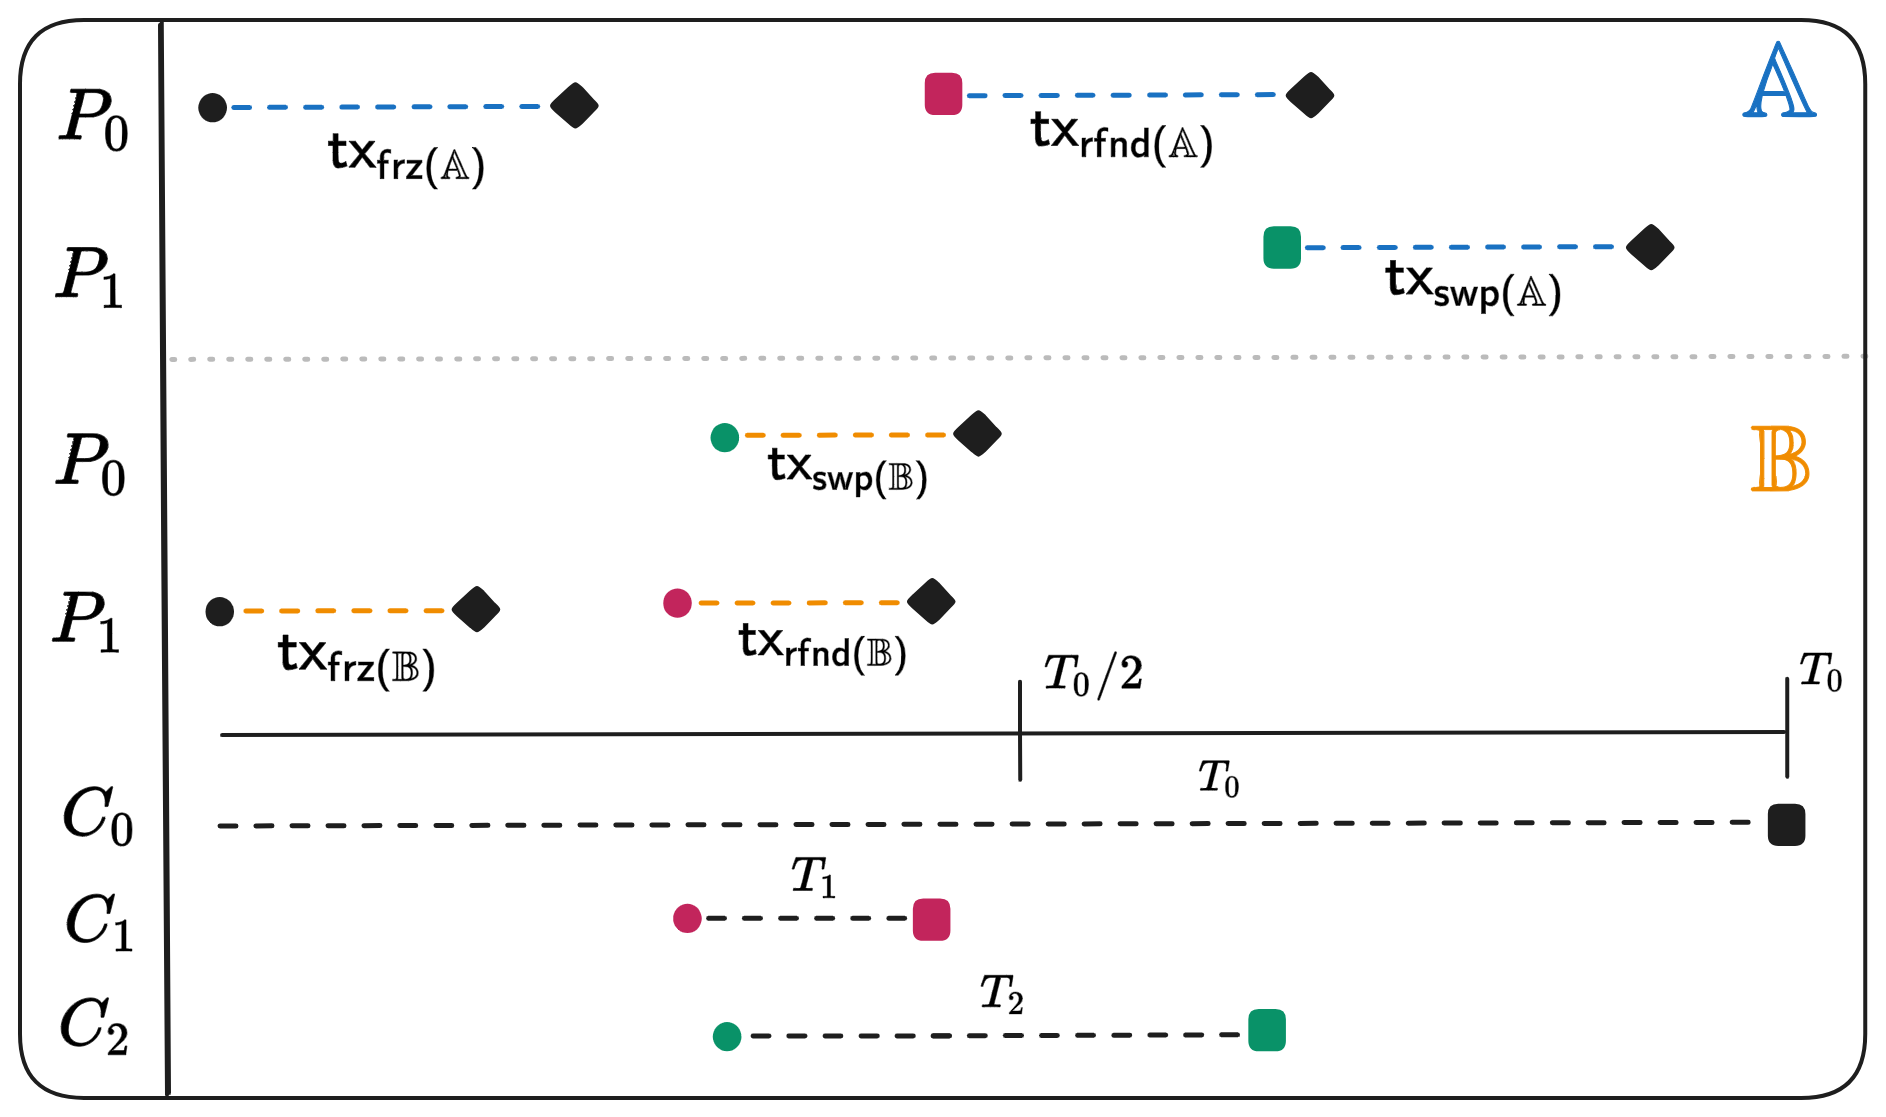
\includegraphics[width=0.8\textwidth]{timeouts.png}
    \caption{Transaction racing between  $\mathsf{tx_{swp(\mathbb{B})}}$ and $\mathsf{tx_{rfnd(\mathbb{B})}}$}
\end{figure}
After the parties run 2PC $\Gamma_{\mathsf{Swap}}$ $P_0$ receives the signature on the swap transaction $\mathsf{tx_{swp(\mathbb{B})}}$. It can then proceed to wait until $P_1$ posts the refund $\mathsf{tx_{rfnd(\mathbb{B})}}$ and then immediately post $\mathsf{tx_{swp(\mathbb{B})}}$ and start force opening $C_1$, which can be retrieved using the refund signature with $C_1 := \mathsf{lk_0} \oplus \sigma_{\mathsf{tx_{rfnd(\mathbb{B})}}}$. On time $T_1$ the force opening completes and $P_0$ proceeds to sign and publish $\mathsf{tx_{rfnd(\mathbb{A})}}$.

Since only $\mathsf{tx_{swp(\mathbb{B})}}$ or $\mathsf{tx_{rfnd(\mathbb{B})}}$ will be confirmed on $\mathbb{B}$, with roughly probability $\frac{1}{2}$, $P_0$ breaks the atomicity property if the former is confirmed as they also obtain $\mathsf{sk_{frz1(\mathbb{A})}}$ from $C_1$ before $P_0$ and can thus successfully complete $\mathsf{tx_{rfnd(\mathbb{A})}}$. \\
Note that $P_1$ can only obtain $\mathsf{sk_{frz1(\mathbb{A})}}$ from $C_2$ after $T_2$, which is strictly later than $T_1$. Inversely, if $T_2 < T_1$, $P_1$ can potentially cheat from the protocol in a similar fashion, performing a racing refund on $\mathbb{B}$ and swapping on $\mathbb{A}$ after they force open $\mathsf{sk_{frz1(\mathbb{A})}}$ from $C_2$. If the time gap between $T_2$ and $T_1$ is smaller than the blockchain's confirmation times, then both sides can potentially try to perfom a racing transaction.

\newpage 
\subsection{Racing transactions in Universal Atomic Swaps}


\begin{figure}[H]
    \centering
    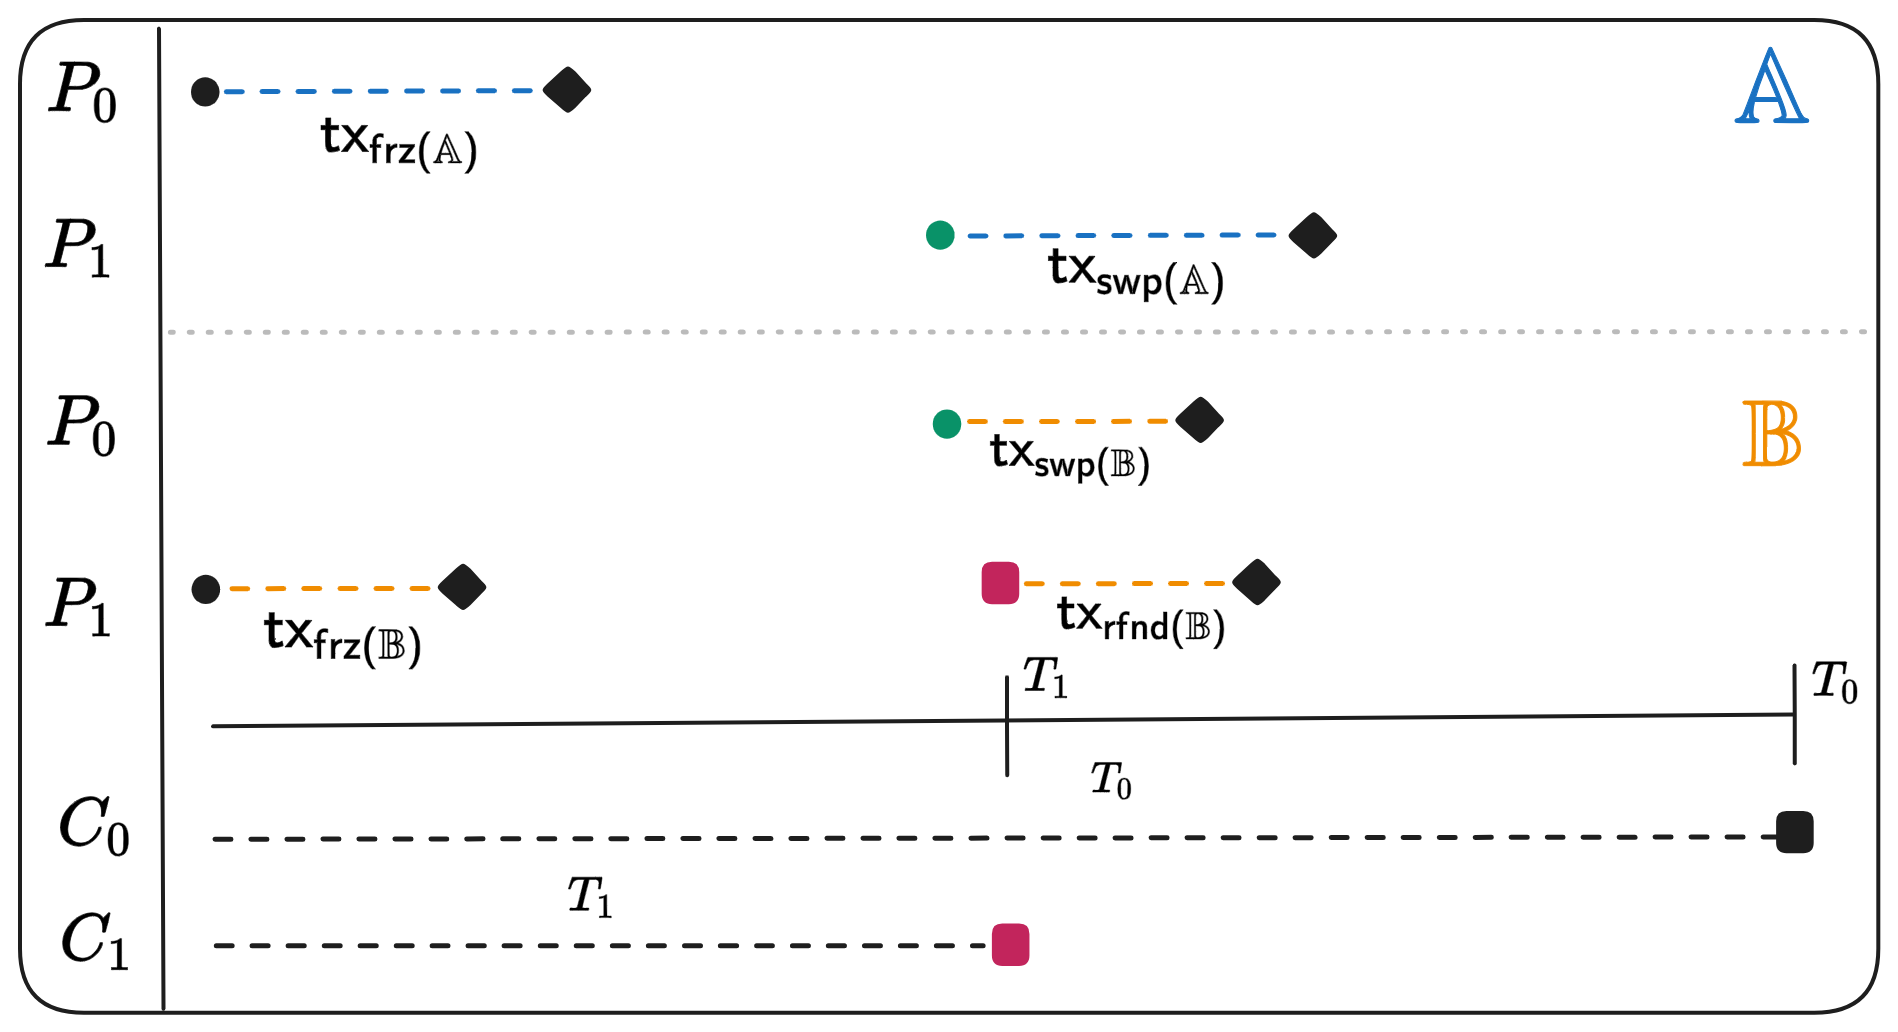
\includegraphics[width=0.8\textwidth]{timeouts-uas.png}
    \caption{Example of a transaction racing condition when $P_0$ posts $\mathsf{tx_{swp(\mathbb{B})}}$ after $T_1 - \mathbb{B}.\mathsf{ctime}$}
\end{figure}

The protocol presented by Thyagarajan et al. \cite{uas} fails to consider two possible transaction racing conditions: \\
1) $P_0$ can wait until $T_1$ to post $\mathsf{tx_{swp(\mathbb{B})}}$, resulting in a transaction racing with $P_1$ posting the refund transaction $\mathsf{tx_{rfnd(\mathbb{B})}}$. Since $\mathsf{tx_{rfnd(\mathbb{B})}}$ is not confirmed until $\mathbb{B}.\mathsf{ctime}$, there is an equal probability that $\mathsf{tx_{swp(\mathbb{B})}}$ will succeed, preventing $P_1$ from refunding the assets. \\
2) Similarly, if $P_0$ posts $\mathsf{tx_{swp(\mathbb{B})}}$ after $T_1 - \mathbb{B}.\mathsf{ctime}$, $P_1$ can simultaneously post $\mathsf{tx_{rfnd(\mathbb{B})}}$ and $\mathsf{tx_{swp(\mathbb{A})}}$, which can result in $P_1$ obtaining both $\mathsf{amnt_a}$ and $\mathsf{amnt_b}$. \\

In order to preserve the atomicity property, we propose the following changes: \\
1) When $P_1$ timeouts at $T_1$, the party should check if $P_0$ is publishing $\mathsf{tx_{swp(\mathbb{B})}}$ while $\mathsf{tx_{rfnd(\mathbb{B})}}$ is unconfirmed. If so, retrieve $\sigma_{swp(\mathbb{A})}$ and publish $\mathsf{tx_{swp(\mathbb{A})}}$. It is also required that $\Delta > \mathbb{A}.\mathsf{ctime} + \mathbb{B}.\mathsf{ctime}$ \\
2) Require $P_0$ to post $\mathsf{tx_{swp(\mathbb{B})}}$ no later than $T_1 - \mathbb{B}.\mathsf{ctime}$, and abort otherwise 

We present the revised protocol in figure 7.

\begin{figure}[H]
\begin{pchstack}[center, boxed]
\pseudocode{
    P_0(\mathsf{sk_{frz0(\mathbb{B})}}, \mathsf{tx_{swp}}) \< \< P_1(\mathsf{sk_{frz1(\mathbb{B})}}) \\[0.1\baselineskip ][\hline] 
    \<\< \\[-0.5\baselineskip ]
    \mathsf{\textbf{if}} \:\: \mathsf{tx_{swp}}.\mathsf{amnt} \neq \mathsf{amnt_b} \\
    \qquad \mathsf{\textbf{return}} \perp \\
    \mathsf{sk_{frz}} := \mathsf{sk_{frz0}} + \mathsf{sk_{frz1}} \\
    \sigma_\mathsf{swp(\mathbb{B})} \gets \Pi_{\mathsf{DS(\mathbb{B})}}.\mathsf{Sign}(\mathsf{sk_{frz}}, \mathsf{tx_{swp}}) \\
    \mathsf{lk} := \mathsf{sk_{frz0}} \oplus \mathsf{\sigma_\mathsf{swp(\mathbb{B})}}  \\
}
\end{pchstack}
\caption{Protocol definition of 2PC $\Gamma_{\mathsf{Swap}}$}
\end{figure}

\begin{figure}[H]
\begin{minipage}[t]{0.5\textwidth}
\begin{pchstack}[boxed]
\pseudocode{
    \text{Global input} \:\: (T_0, T_1, \mathsf{amnt_a}, \mathsf{amnt_b},\mathbb{A}, \mathbb{B}) \\[0.1\baselineskip ][\hline] \\
    (\mathsf{sk_{frz0}}, \mathsf{pk_{frz}})_{(\mathbb{A})} \gets \mathsf{\textbf{wait}} \:\: \Gamma_{\mathsf{KeyGen}_{(\mathbb{A})}} \\
    (\mathsf{sk_{frz1}}, \mathsf{pk_{frz}})_{(\mathbb{B})} \gets \mathsf{\textbf{wait}} \:\: \Gamma_{\mathsf{KeyGen}_{(\mathbb{B})}} \\
    (C_1, \pi_1) \gets \Pi_\mathsf{VTD}.\mathsf{Commit}(\mathsf{sk_{frz0(\mathbb{A})}}, T_1) \\
    (C_0, \pi_0) \gets \mathsf{\textbf{wait}} \:\: \mathsf{receive}(P_1) \\
    \mathsf{\textbf{wait}} \:\: \mathsf{send}(P_1,\: (\pi_1, C_1) \\
    \mathsf{\textbf{if}} \:\: \Pi_{\mathsf{VTD}}.\mathsf{Verify}({[\mathsf{sk_{frz1(\mathbb{A})}}]}, C_0, \pi_0) \neq 1 \\
        \quad \mathsf{\textbf{return}} \perp \\
    mathsf{\textbf{select}} \:\: \{ \\
        \quad \mathsf{\textbf{wait}} \:\: \{ \\
            \qquad \mathsf{sk_{frz1}} \gets \Pi_{\mathsf{VTD}}.\mathsf{ForceOp}(C_0) \\
            \qquad \mathsf{sk_{frz(\mathbb{A})}} := \mathsf{sk_{frz0}} + \mathsf{sk_{frz1}} \\
            \qquad \mathsf{FullTx}_{(\mathbb{A})}(\mathsf{pk_{frz}}, \mathsf{pk_{init}}, \mathsf{amnt_a}, \mathsf{sk_{frz}}) \\
        \quad \} \\
        \quad \mathsf{\textbf{wait}} \:\: \{ \\
        \qquad \mathsf{FullTx}_{(\mathbb{A})}(\mathsf{pk_{init}}, \mathsf{pk_{frz}}, \mathsf{amnt_a}, \mathsf{sk_{init}}) \\
            \qquad \mathsf{\textbf{do}} \:\: \mathsf{bal_b} \gets \mathbf{wait} \:\: \mathsf{GetBal}_{(\mathbb{B})}(\mathsf{pk_{frz}}) \\
            \qquad \mathsf{\textbf{while}} \:\: \mathsf{bal_b} \neq {\mathsf{amnt_b}} \\
\
            \qquad \sigma_{\mathsf{swp(\mathbb{B})}} \gets \Gamma_{\mathsf{Swap}}(\mathsf{sk_{frz0(\mathbb{B})}}, \mathsf{tx_{swp(\mathbb{B})}}) \\
            \qquad \textbf{if} \:\: \mathsf{VerifyTx}_{(\mathbb{B})}(\sigma_{\mathsf{swp}}, \mathsf{tx_{swp}}) \neq 1 \\
            \qquad \quad \mathsf{\textbf{return}} \perp \\
            \qquad \textbf{if} \:\: \mathsf{GetTime}() > T_1 - \mathbb{B}.\mathsf{ctime} \\
            \qquad \quad \mathsf{\textbf{return}} \perp \\
            \qquad \mathsf{PubTx}_{(\mathbb{B})}(\sigma_{\mathsf{swp}}, \mathsf{tx_{swp}}) \\
            \qquad \mathsf{WatchTx}_{(\mathbb{B})}(\sigma_{\mathsf{swp}}, \mathsf{tx_{swp}}) \\
        \quad \} \\
    \}
}
\end{pchstack}
\end{minipage}%
\begin{minipage}[t]{0.5\textwidth}
\begin{pchstack}[boxed]
\pseudocode{
    \text{Global input} \:\: (T_0, T_1, \mathsf{amnt_a}, \mathsf{amnt_b},\mathbb{A}, \mathbb{B}) \\[0.1\baselineskip ][\hline] \\
    (\mathsf{sk_{frz1}}, \mathsf{pk_{frz}})_{(\mathbb{A})} \gets \mathsf{\textbf{wait}} \:\: \Gamma_{\mathsf{KeyGen}_{(\mathbb{A})}} \\
    (\mathsf{sk_{frz1}}, \mathsf{pk_{frz}})_{(\mathbb{B})} \gets \mathsf{\textbf{wait}} \:\: \Gamma_{\mathsf{KeyGen}_{(\mathbb{B})}} \\
    (C_0, \pi_0) \gets \Pi_\mathsf{VTD}.\mathsf{Commit}(\mathsf{sk_{frz1(\mathbb{A})}}, T_0) \\
    \mathsf{\textbf{wait}} \:\: \mathsf{send}(P_0,\: (C_0, \pi_0) \\
    (C_1, \pi_1) \gets \mathsf{\textbf{wait}} \:\: \mathsf{receive}(P_1) \\
    \mathsf{\textbf{if}} \:\: \Pi_{\mathsf{VTD}}.\mathsf{Verify}({[\mathsf{sk_{frz0(\mathbb{A})}}]}, C_1, \pi_1) \neq 1 \\
        \quad \mathsf{\textbf{return}} \perp \\
    \mathsf{\textbf{select}} \:\: \{ \\
        \quad \mathsf{\textbf{wait}} \:\: \{ \\
            \qquad \mathsf{sk_{frz0}} \gets \Pi_{\mathsf{VTD}}.\mathsf{ForceOp}(C_1) \\
            \qquad \mathsf{sk_{frz(\mathbb{B})}} := \mathsf{sk_{frz0}} + \mathsf{sk_{frz1}} \\
            \qquad \mathsf{FullTx}_{(\mathbb{B})}(\mathsf{pk_{frz}}, \mathsf{pk_{init}}, \mathsf{amnt_b}, \mathsf{sk_{frz}}) \\
        \quad \} \\
        \quad \mathsf{\textbf{wait}} \:\: \{ \\
            \qquad \mathsf{FullTx}_{(\mathbb{B})}(\mathsf{pk_{init}}, \mathsf{pk_{frz}}, \mathsf{amnt_b}, \mathsf{sk_{init}}) \\
            \qquad \mathsf{\textbf{do}} \:\: \mathsf{bal_a} \gets \mathsf{GetBal}_{(\mathbb{A})}(\mathsf{pk_{frz}}) \\
            \qquad \mathsf{\textbf{while}} \:\: \mathsf{bal_a} \neq {\mathsf{amnt_a}} \\
            \qquad (\mathsf{lk}, \mathsf{hsig}) \gets \Gamma_{\mathsf{Swap}}(\mathsf{sk_{frz1(\mathbb{B})}}) \\
            \qquad \mathsf{\textbf{do}} \:\: (\sigma_\mathsf{tx_{last}}, \_) \gets \mathsf{GetLatestTx}_{(\mathbb{B})}(\mathsf{pk_{frz}}) \\
            \qquad \mathsf{\textbf{while}} \:\: \mathcal{H}(\sigma_\mathsf{tx_{last}}) \neq {\mathsf{hsig}} \\
            \qquad \mathsf{sk_{frz0(\mathbb{A})}} :=  \mathsf{lk} \oplus \mathsf{hsig} \\
            \qquad \mathsf{sk_{frz(\mathbb{A})}} := \mathsf{sk_{frz0}} + \mathsf{sk_{frz1}} \\
            \qquad \mathsf{FullTx}_{(\mathbb{A})}(\mathsf{pk_{frz}}, \mathsf{pk_{swp}}, \mathsf{amnt_a}, \mathsf{sk_{frz}}) \\
        \quad \} \\
    \} \\
}

\end{pchstack}
\end{minipage}%
\caption{Universal Atomic Swap protocol for parties $P_0$ and $P_1$, revised version}
\end{figure}



\section{Open directions}

In this section, we outline several avenues for future research and development that build upon the work presented in this report. These open directions address both theoretical and practical aspects of the topic, suggesting pathways for further exploration and improvement.
\subsection*{One-sided commitments protocols}
The protocol we proposed is susceptible to a potential racing transaction condition, as described in Figure 5. An open question is whether it is possible to construct an atomic swap protocol that employs a one-sided refund commitment while avoiding this issue. 
To explore this, future research could focus on algorithmically identifying alternative protocols by:
\begin{itemize}
        \item Constructing transaction "locks" by masking commitments or secret key shares with transaction signatures or other data
        \item Defining mutual exclusion conditions on the swap transaction ($\mathsf{tx_{swp}}$) and the refund transaction ($\mathsf{tx_{rfnd}}$) happening on the same blockchain
\end{itemize}
By establishing these conditions and systematically evaluating protocols across all possible combinations of transaction locks, it may be possible to verify whether such a protocol can be successfully realized, or alternatively, to prove the infeasibility of such.

\subsection*{Further improvements and implementation}
The $\mathsf{VTS}$ scheme presented  by Thyagarajan et al. \cite{vts} suffers from time unverifiability, that is a proof $\pi$ from $\mathsf{VTD}.\mathsf{Commit}$ does not in fact prove that the resulting commitment $C$ can be opened in $T$ steps. However, improving on the work of \cite{vts}, Zhou et al. \cite{fixed_vts} have proposed an extension to verifiable timed commitment that offers \textit{verifiable timed recovery}, that is, the recipient can verify that the forced open algorithm returns a valid value after time $T$.

Furthermore, $\mathsf{VTS}$ schemes require a trusted setup, and it is unclear how the authors of Universal Atomic Swaps \cite{uas} address this operation in a Peer-to-Peer setting. \\
We note that the version of Universal Atomic Swaps that we presented in this work uses a $\mathsf{VTD}$ scheme as opposed to $\mathsf{VTS}$ in order to be compatible with blockchains that do not support \textit{transaction chaining} and \textit{pre-signatures}, such as Monero \cite{pre_sign}. \\
To the best of our knowledge, only the building blocks used in the protocol have been implemented, while a full protocol implementation is missing.

\subsection*{Evaluating computational advantages in solving timelock puzzles}
In order to guarantee security of the protocol, parties need to set timeouts with worst-case estimates for the available computational power. A precise evaluation of the speedup offered for sequential squaring using ASICs \cite{squaring_asic} over conventional hardware is thus critical in order to argument the practicality of the protocol.

\subsection*{Commit transactions}
A blockchain functionality equivalent to HTLCs but that does not require general scripting capabilities can be easily realized in \textit{public} ledgers, as defined in the appendix. However, realizing such a construction in private blockchains that use privacy-preserving transaction schemes such as RingCT \cite{ring_signatures} in Monero or zk-SNARKs based shielded addresses in Zcash \cite{zcash} is non-trivial and should be subject of further research.

\newpage
\printbibliography

\newpage

\appendix


\section*{Appendix}
\subsection*{Commit transaction}

Commit transactions can be easily realized by a blockchain using a public ledger model by modifying consensus rules, and require no additional scripting capabilities.  \\
A commit transaction allows to lock assets for a specified transfer until a certain timeout T, commiting to a secret value $x$ in $C$. If $C$ gets opened by broadcasting the revealed $x$ before timeout T, the transfer is completed unconditionally. \\ 
After timeout T, the commit transaction is considered expired, unfreezing the assets and ignoring openings on $C$.

We further define the following routines for blockchains that support commitment transaction.
\begin{itemize}[topsep=0pt, itemsep=0pt, leftmargin=2em]
	\item $\mathbf{ctx}_{\mathbb{A}} := (\mathsf{tx_{\mathbb{A}}}, C) \gets \mathbf{CommitTx}_{(\mathbb{A})}(C, \mathsf{pk_{tx}}, \mathsf{pk_{rx}}, \mathsf{amnt}, \mathsf{T})$: creates an unsigned commit transaction paying $\mathsf{amnt}$ from $\mathsf{pk_{tx}}$ to $\mathsf{pk_{rx}}$ valid until time $\mathsf{T}$, whith  $\mathsf{amnt}$ being locked from being spent on transactions from $\mathsf{pk_{tx}}$ until $\mathsf{T}$. The transaction can be later finalized by opening and broadcasting $C$ through $\mathsf{RevTx}$.
\item $ \mathbf{0/1} \gets \mathbf{RevTx}_{(\mathbb{A})}(\mathsf{sec}, \mathsf{ctx})$: open the (on-chain) committed transaction $\mathsf{ctx}$ by revealing the commited secret $\mathsf{sec}$. Return 0 if the opening fails or the timeout on $\mathsf{ctx}$ has expired. If the revealing succeeds, return 1 and finalize $\mathsf{ctx}$.
\end{itemize}

By assuming this functionality on both chains we can now realize the following atomic swap protocol.

\begin{figure}[H]
\begin{minipage}[t]{0.5\textwidth}
\begin{pchstack}[boxed]
\pseudocode{
    \text{Global input} \:\: (T, \mathsf{amnt_a}, \mathsf{amnt_b},\mathbb{A}, \mathbb{B}) \\[0.1\baselineskip ][\hline] \\
    \mathsf{sec} \gets \mathbb{Z}_q \\
    (C_0, r) \gets \Pi_{\mathsf{PCom}}.\mathsf{Commit}(\mathsf{sec_0}) \\ % verify that sec_0 has been commited
    \mathsf{ctx_{(\mathbb{A})}} \gets \mathsf{CommitTx}_{(\mathbb{A})}(C_0, \mathsf{pk_{init}}, \mathsf{pk_{swp}}, \mathsf{amnt_a}, T + \Delta) \\
    \sigma_{\mathsf{ctx_{(\mathbb{A})}}} \gets \Pi_{\mathsf{DS(\mathbb{A})}}.\mathsf{Sign}(\mathsf{sk_{init}}, \mathsf{ctx}) \\
    \mathsf{PubTx}_{(\mathbb{A})}(\sigma_{\mathsf{ctx}}, \mathsf{ctx}) \\
    \mathsf{\textbf{select}} \:\: \{ \\
    \quad \mathsf{\textbf{wait}} \:\: \{ \\
    \qquad \mathsf{timeout}(T) \\
    \quad \} \\
    \quad \mathsf{\textbf{wait}} \:\: \{ \\
    \qquad \mathsf{send}(\mathsf{ctx_{(\mathbb{A})}}) \\
    \qquad \mathsf{receive}(\mathsf{ctx_{(\mathbb{B})}}) \\
    \qquad \mathsf{res_1} \gets \mathsf{\textbf{wait}} \:\: \mathsf{WatchTx}_{(\mathbb{B})}(\mathsf{ctx}) \\
    \qquad \mathsf{\textbf{if}} \:\: \mathsf{ctx}_{(\mathbb{B})}.C \neq C_0 \lor \mathsf{ctx}_{(\mathbb{B})}.T \neq T \lor \mathsf{res_1} \neq 1 \\ % verify that commit transaction is valid and accepted
    \qquad \quad \mathsf{\textbf{return}} \perp \\
    \qquad \mathsf{rtx_{swp(\mathbb{B})}} \gets \mathsf{RevTx}_{(\mathbb{B})}(\mathsf{sec}, \mathsf{ctx}) \\
    \quad \} \\
    \} \\
}
\end{pchstack}
\end{minipage}%
\hspace{0.4cm}
\begin{minipage}[t]{0.5\textwidth}
\begin{pchstack}[boxed]
\pseudocode{
    \text{Global input} \:\: (T, \mathsf{amnt_a}, \mathsf{amnt_b},\mathbb{A}, \mathbb{B}) \\[0.1\baselineskip ][\hline] \\
    \mathsf{receive}(\mathsf{ctx_{(\mathbb{A})}}) \\
    \mathsf{res_0} \gets \mathsf{\textbf{wait}} \:\: \mathsf{WatchTx}_{(\mathbb{A})}(\mathsf{ctx}) \\
    \mathsf{\textbf{select}} \:\: \{ \\
    \quad \mathsf{\textbf{wait}} \:\: \{ \\
    \qquad \mathsf{timeout}(T) \\
    \quad \} \\
    \quad \mathsf{\textbf{wait}} \:\: \{ \\
    \qquad \mathsf{\textbf{if}} \:\: \mathsf{ctx_{(\mathbb{A})}}.T \neq T + \Delta \lor \mathsf{res_0} \neq 1 \\ % verify that commit transaction is valid and accepted
    \qquad \quad \mathsf{\textbf{return}} \perp \\
    \qquad \mathsf{ctx}_{(\mathbb{B})} \gets \mathsf{CommitTx}_{(\mathbb{B})}(C_0, \mathsf{pk_{init}}, \mathsf{pk_{swp}}, \mathsf{amnt_b}, T) \\
    \qquad \mathsf{send}(\mathsf{ctx}_{(\mathbb{B})}) \\
    \qquad \mathsf{rtx_{swp(\mathbb{B})}} \gets \mathsf{\textbf{wait}} \:\: \mathsf{GetLatestTx}_{(\mathbb{B})}(\mathsf{pk_{swp}}) \\
    \qquad \mathsf{sec} := \mathsf{rtx_{swp(\mathbb{B})}}.\mathsf{rev} \\
    \qquad \mathsf{rtx_{swp(\mathbb{A})}} \gets \mathsf{RevTx}_{(\mathbb{A})}(\mathsf{sec}, \mathsf{ctx}) \\
    \quad \} \\
    \} \\
}
\end{pchstack}
\end{minipage}%
\caption{Full protocol execution for $P_0$ and $P_1$, respectively left and right}
\end{figure}


\end{document}
